\chapter{水下机器人系统建模与仿真}

\section{引言}
查找文献下,写一些水下机器人分类,控制系统跟动力学运动学的关系,引用参考文献。

\section{运动学模型和非完整约束}

通过考虑线速度的非完整约束,得到了系统的运动学模型\cite{ref20}。
非完整约束将系统在某些方向上的速度限制为零,但这些限制并不限制系统的全局运动\cite{ref19}。
当两个表面相互滚动时,或者在系统的总角动量守恒的天基系统中,就会出现这种约束\cite{ref29}。
为了建立水下AUV的运动学模型\cite{ref25},我们假设两个正交坐标系,全局坐标和本体坐标,如\autoref{fig:3-1}所示。

\begin{figure}[htbp]
    \centering
    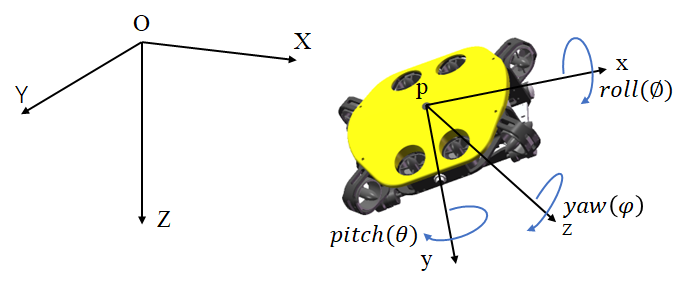
\includegraphics[width=14.5cm]{毕设图片/3-1.png}
    \caption{\label{fig:3-1}水下机器人坐标系}
\end{figure}
假如不考虑$y跟z$方向上的运动,此时
AUV运动学模型有六个状态变量和四个输入变量。
描述两者之间关系转换的运动学坐标系可以用很多个参数表示,以下运动学模型是用欧拉角的方法建立的\cite{ref21}。
\begin{equation}
    \begin{split}
        \label{equ:3-1}
    &R=\begin{bmatrix}r_{11}&r_{12}&r_{13}\\r_{21}&r_{22}&r_{23}\\r_{31}&r_{32}&r_{33}\end{bmatrix}=\begin{bmatrix}n&s&a\end{bmatrix}\\
    &r_{11}=\cos\:\theta\cos\:\psi\\
    &r_{12}=\sin\:\theta\sin\:\phi\cos\:\psi-\cos\:\phi\sin\:\psi\\
    &r_{13}=\sin\:\theta\cos\:\phi\cos\:\psi\\
    &r_{21}=\cos\:\theta\sin\:\psi\\
    &r_{22}=\sin\:\theta\sin\:\phi\sin\:\psi+\cos\:\phi\cos\:\psi\\
    &r_{23}=\sin\:\theta\cos\:\phi\sin\:\psi-\sin\:\phi\cos\:\psi\\
    &r_{31}=-\sin\:\theta\\
    &r_{32}=\sin\:\phi\cos\:\theta\\
    &r_{33}=\cos\:\phi\cos\:\theta
    \end{split}
\end{equation}
式子中,$\phi$ 是横滚角,$\theta $是俯仰角,$\psi $是偏航角,$R$是绕$xyz$旋转的旋转矩阵,$R$是正交单位矩阵,满足$RR^T = I, R^T = R^{-1},det(R) = 1$。
令:

\begin{equation}
    p=\begin{bmatrix}{x}\\{y}\\{z}\end{bmatrix},
    \eta=\begin{bmatrix}\phi\\\theta\\\psi\end{bmatrix},
    {q}=\begin{bmatrix}p\\\\\eta\end{bmatrix}
\end{equation}
\begin{equation}
    \\v=
    \begin{bmatrix}v_{x}\\0\\0\end{bmatrix}, 
    \omega=\begin{bmatrix}\omega_{x}\\\omega_{y}\\
        \omega_{z}
    \end{bmatrix} 
\end{equation}
式中,$p$是本体坐标原点在全局坐标系下的坐标,$\eta$是欧拉角,$v$是本体坐标系下AUV的速度,$\omega$是本体坐标系下AUV的角速度。使用旋转矩阵可以得到\cite{ref22}:
\begin{equation}
    \dot{p} = Rv 
\end{equation}
定义两个向量:
\begin{equation}
    a=\begin{bmatrix}a_1\\a_2\\a_3\end{bmatrix}=a_1i+a_2j+a_3k,b=\begin{bmatrix}b_1\\b_2\\b_3\end{bmatrix}=b_1i+b_2j+b_3k
\end{equation}
\begin{equation}
    i=\begin{bmatrix}1\\0\\0\end{bmatrix},j=\begin{bmatrix}0\\1\\0\end{bmatrix},k=\begin{bmatrix}0\\0\\1\end{bmatrix}
\end{equation}
利用向量叉乘的定义可以得到:
\begin{equation}  
\text{a×b} =(a_2b_3-a_3b_2)i+(a_3b_1-a_1b_3)j+(a_1b_2-a_2b_1)k 
\end{equation}
即:
\begin{equation}  
    a\times b =\begin{vmatrix}i&j&k\\a_1&a_2&a_3\\b_1&b_2&b_3\end{vmatrix} 
 \end{equation}
 把叉乘转化为矩阵相乘的形式可以得到:
 \begin{equation}
    a\times b=[a\times]b=\begin{bmatrix}0&-a_3&a_2\\a_3&0&-a_1\\-a_2&a_1&0\end{bmatrix}\begin{bmatrix}b_1\\b_2\\b_3\end{bmatrix}
\end{equation}
 所以得到一个定义:
 \begin{equation}
    [a\times]=\begin{bmatrix}0&-a_3&a_2\\a_3&0&-a_1\\-a_2&a_1&0\end{bmatrix}
\end{equation}
对于刚体上的任意固定一点$x_0$,转换后在全局坐标系下的坐标为$\mathrm{X}(t)$,则
\begin{equation}
    \mathrm{X}(t)=Rx_0
\end{equation}
对等式两边同时求导可以得到:
\begin{equation}
    \dot{X}=\dot{R}x_0+R\dot{x_0}
\end{equation}
由于$x_0$是一个固定的点,所以 $\dot{x_0}=0$,所以化简上式可以得到:
\begin{equation}
    \mathrm{V}=\dot{R}x_0=Rv=Rw\times x_0
\end{equation}
式中$\mathrm{V}$代表AUV在本体坐标系下的速度。进一步化简上式子可以得到:
\begin{equation}
    \label{equ:3-14}
   \dot{R}=\mathrm{RS}(\omega)
\end{equation}
\begin{equation}
    S(\omega)=\begin{bmatrix}0&-\omega_z&\omega_y\\\omega_z&0&-\omega_x\\-\omega_y&\omega_x&0\end{bmatrix}
\end{equation}
令:
\begin{equation}
    \dot{p}=J_1(\eta)v,\dot{\eta}=J_2(\eta)\omega 
\end{equation}
显而易见,可以得出如下公式:
\begin{equation}
    J_{1}(\eta)=[\cos\theta\cos\psi\quad\cos\theta\sin\psi\quad-\sin\theta]^{T}
\end{equation}
根据旋转矩阵的定义可以得到:
\begin{equation}
    \begin{aligned}
&R=R_{xyz}=R_zR_yR_x \\
&=\begin{pmatrix}\cos\phi&-\sin\phi&0\\\sin\phi&\cos\phi&0\\0&0&1\end{pmatrix}\begin{pmatrix}\cos\theta&0&\sin\theta\\0&1&0\\-\sin\theta&0&\cos\theta\end{pmatrix}\begin{pmatrix}1&0&0\\0&\cos\psi&-\sin\psi\\0&\sin\psi&\cos\psi\end{pmatrix}
\end{aligned}
\end{equation}
R对时间求偏导,对于上述式子可以转化为对时间的全导数,得到:
\begin{equation}
    \frac{\mathrm{d}R}{\mathrm{d}t}=\frac{\mathrm{d}\left(R_zR_pR_x\right)}{\mathrm{d}t}=\frac{\mathrm{d}R_z}{\mathrm{d}t}R_yR_x+R_z\frac{\mathrm{d}R_y}{\mathrm{d}t}R_x+R_zR_y\frac{\mathrm{d}R_x}{\mathrm{d}t}
\end{equation}
同时可以得到:
\begin{equation}
    \begin{gathered}
\frac{dR_z}{dt} =\begin{pmatrix}0&0&0\\0&-\sin \psi&-\cos \psi\\0&\cos \psi&-\sin \psi\end{pmatrix}\frac{\mathrm{d}\psi}{\mathrm{d}t} \\
\frac{\mathrm{d}R_y}{\mathrm{d}t} =\begin{pmatrix}-\sin \theta&0&\cos \theta\\0&0&0\\-\cos \theta&0&-\sin \theta\end{pmatrix}\frac{\mathrm{d}\theta}{\mathrm{d}t} \\
\frac{\mathrm{d}R_x}{\mathrm{d}t} =\begin{pmatrix}-\sin \phi&-\cos \phi&0\\\cos \phi&-\sin \phi&0\\0&0&0\end{pmatrix}\frac{\mathrm{d}\phi}{\mathrm{d}t} 
\end{gathered}
\end{equation}
由\autoref{equ:3-14}和$R$的性质可以得到:
\begin{equation}
    \begin{aligned}
        \label{equ:3-21}
&S(\omega)=R^\mathrm{T}\frac{\mathrm{d}R}{\mathrm{d}t} \\
&=R_x^TR_y^TR_z^T\left(\frac{\mathrm{d}R_z}{\mathrm{d}t}R_yR_x+R_z\frac{\mathrm{d}R_y}{\mathrm{d}t}R_x+R_zR_y\frac{\mathrm{d}R_x}{\mathrm{d}t}\right) \\
&=R_x{}^TR_y{}^TR_z^T\frac{\mathrm{d}R_z}{\mathrm{d}t}R_yR_x+R_x{}^TR_y{}^T\frac{\mathrm{d}R_y}{\mathrm{d}t}R_x+R_x{}^T\frac{\mathrm{d}R_x}{\mathrm{d}t}
\end{aligned}
\end{equation}
又因为:
\begin{equation}
    \label{equ:3-22}
    S(\omega)=\begin{bmatrix}0&-\omega_z&\omega_y\\\omega_z&0&-\omega_x\\-\omega_y&\omega_x&0\end{bmatrix}
\end{equation}
将欧拉角导数记为 $\dot{\eta}=(\dot{\psi},\dot{\theta},\dot{\phi})^{T}$,
由\autoref{equ:3-21}和\autoref{equ:3-22}可以得到
 $\dot{\eta}$与$\omega$的关系式,经过计算可以得出:
 \begin{equation}
    J_2(\eta)=\begin{bmatrix}1&\sin\phi\tan\theta&\cos\phi\tan\theta\\0&\cos\phi&-\sin\phi\\0&\sin\phi\sec\theta&\cos\phi\sec\theta\end{bmatrix}
\end{equation}

所以最后得出\cite{ref23}:
\begin{equation}
    \begin{aligned}
&\dot{x}(t) =r_{11}v=\cos\psi\text{cos }\theta v \\
&\dot{y}(t) =r_{21}v=\sin \psi\text{cos }\theta v \\
&\dot{z}(t) =r_{31}v=-\sin \theta v \\
&\dot{\phi}(t) =\omega_x+\sin^2\phi\tan^2\theta\omega_y+\cos^2\phi\tan^2\theta\omega_z \\
&\dot{\theta}(t) =\cos^2\phi\omega_y-\sin^2\phi\omega_z \\
&\dot{\psi}(t) =\sin \phi\sec \theta\omega_y+\cos \phi\sec \theta\omega_z 
\end{aligned}
\end{equation}
写成矩阵的形式为:
\begin{equation}
    \begin{bmatrix}\dot{x}(t)\\\dot{y}(t)\\\dot{z}(t)\\\dot{\phi}(t)\\\dot{\theta}(t)\\\dot{\psi}(t)\end{bmatrix}=\begin{bmatrix}\cos\psi\cos\theta&0&0&0\\\sin\psi\cos\theta&0&0&0\\-\sin\theta&0&0&0\\0&1&\sin\phi\tan\theta&\cos\phi\tan\theta\\0&0&\cos\phi&-\sin\phi\\0&0&\sin\phi\sec\theta&\cos\phi\sec\theta\end{bmatrix}\begin{bmatrix}v\\\omega_x\\\omega_y\\\omega_z\end{bmatrix}
\end{equation}
也可以写成如下形式:
\begin{equation}
    \begin{bmatrix}\dot{x}(t)\\\dot{y}(t)\\\dot{z}(t)\\\dot{\phi}(t)\\\dot{\theta}(t)\\\dot{\psi}(t)\end{bmatrix}=\begin{bmatrix}\cos\psi\cos\theta\\\sin\psi\cos\theta\\-\sin\theta\\0\\0\\0\end{bmatrix}v+\begin{bmatrix}0\\0\\0\\1\\0\\0\end{bmatrix}\omega_x+\begin{bmatrix}0\\0\\0\\\sin\phi\tan\theta\\\cos\phi\\\sin\phi\sec\theta\end{bmatrix}\omega_y+\begin{bmatrix}0\\0\\0\\\cos\phi\tan\theta\\-\sin\phi\\\cos\phi\sec\theta\end{bmatrix}\omega_z
\end{equation}
因为此种情况下水下机器人只沿着本体坐标系x轴移动,所以系统有两个约束,即:
\begin{equation}
    \begin{aligned}
    s^T\dot{p}=0,\quad r_{12}\dot{x}+r_{22}\dot{y}+r_{32}\dot{z}=0
    \\a^T\dot{p}=0,\quad r_{13}\dot{x}+r_{23}\dot{y}+r_{33}\dot{z}=0
\end{aligned} 
\end{equation}
把参数带入可以得到:
\begin{equation}
    \begin{aligned}
        \begin{bmatrix}\cos \psi\sin \theta\sin \phi-\sin \psi\cos \phi
            &\sin \psi\sin \theta\sin \phi+\cos \psi\cos \phi
            &\cos \theta\sin \phi
            \\\sin \psi\sin \theta\cos \phi-\sin \psi\sin \phi
            &\sin \psi\sin \theta\cos \phi-\cos \psi\sin \phi
            &\cos \theta\cos \phi\end{bmatrix}\begin{bmatrix} \dot{x}
                \\\dot{y}\\\dot{z}
            \end{bmatrix}=0
\end{aligned}     
\end{equation}
写成如下简洁形式可得:
\begin{equation}
    A(q)\dot{q}=0 
\end{equation}
\begin{equation}
    \begin{aligned}
A(q)=\begin{bmatrix}r_{12}&r_{22}&r_{32}&0&0&0\\r_{13}&r_{23}&r_{33}&0&0&0\end{bmatrix}
\end{aligned}   
\end{equation}
整理上面结果可以得到:
\begin{equation}
    \dot{q}(t)=g_1(q)v_1+g_2(q)v_2+g_3(q)v_3+g_4(q)v_4
\end{equation}
\begin{equation}
    \dot{q}(t)=[g_1(q)\quad g_2(q)\quad g_3(q)\quad g_4(q)]\begin{bmatrix}v_1\\v_2\\v_3\\v_4\end{bmatrix}
\end{equation}
\begin{equation}
    v_1=v_x;v_2=\omega_x;v_3=\omega_y;v_4=\omega_z;v_p = \begin{bmatrix}v_1\\v_2\\v_3\\v_4\end{bmatrix}
\end{equation}
\begin{equation}
    \begin{aligned}
&g_{1}(q) =[\cos\theta\cos\psi\quad\cos\theta\sin\psi\quad-\sin\theta\quad0\quad0\quad0]^T \\
&g_2(q) =[\begin{matrix}0&0&0&1&0&0\end{matrix}]^T \\
&g_{3}(q) =\begin{bmatrix}0&0&0&\sin\phi\tan\theta&\cos\phi&\sin\phi\sec\theta\end{bmatrix}^T \\
&g_{4}(q) =\begin{bmatrix}0&0&0&\cos\phi\tan\theta&-\sin\phi&\cos\phi\sec\theta\end{bmatrix}^T 
\end{aligned}
\end{equation}
所以此种情况下水下机器人的运动学方程为:
\begin{equation}
    \dot{q}=G(q)v_p
\end{equation}
同理,当水下机器人考虑六自由度运动时,此时 AUV 的运动学模型有六个状态变量和
六个输入变量,此时:
\begin{equation}
    \\v=
    \begin{bmatrix}v_\mathrm{x}\\v_\mathrm{y}\\v_\mathrm{Z}\end{bmatrix}
\end{equation}
可以求得:
\begin{equation}
    \left.\boldsymbol{J}_1(\boldsymbol{\eta}_2)=\left[\begin{array}{ccc}\text{с}\psi c\theta&-s\psi c\phi+c\psi s\phi s\theta&s\psi s\phi+\text{с}\psi c\phi s\theta\\s\psi c\theta&c\psi c\phi+s\psi s\phi s\theta&-c\psi s\phi+s\psi c\phi s\theta\\-s\theta&c\theta s\phi&c\theta c\phi\end{array}\right.\right]
\end{equation}
在上述公式中,为了描述方便,定义:
 $ c = cos() , s = sin(), t = tan()$。

 所以水下机器人六自由度运动学方程为:
 \begin{equation}
     \dot{q}=\begin{bmatrix}J_1\quad O\\ O\quad J_2\end{bmatrix}\begin{bmatrix}v\\\omega\end{bmatrix}
 \end{equation}
 \begin{equation}
    O=\begin{bmatrix}0\quad 0\quad 0\\0\quad 0\quad 0\\0\quad 0\quad 0\end{bmatrix}
\end{equation}
\section{水下机器人动力学模型}
由于航行器所受到刚体动力学与流体动力学作用到本体上具有同时性,可以根据线性系统的等效叠加原理进行动力学建模\cite{ref27}。
因此,将水下机器人的动力学建模主要分为刚体动力学建模与流体动力学建模\cite{ref26}。为了更加清晰的描述水下机器人的运动状态,
对其参数定义进行汇总,如\autoref{tab:3-1}所示
\begin{table}[H]
    \fangsong
    \caption{\label{tab:3-1}水下机器人运动参数定义}
    \small %此处写字体大小控制命令
    \centering%把表居中
    \renewcommand{\arraystretch}{1.5}
    \setlength{\tabcolsep}{3mm}{
    \begin{tabular}{ccccc}
    \toprule%第一道横线位姿 
   & 位姿 & 速度 & 力(矩) \\  参考系  &惯性坐标系 &体坐标系 &体坐标系\\
    \midrule%第二道横线 
    纵荡 &  $x$     & $v_x$ & $X$ \\
    横荡 &	$y$     &	$v_y$ &	$Y$ \\
    垂荡 &	$z $    & $v_z$ &	$Z$\\
    横滚 &	$\phi$  &	$\omega_x$ & $K$ \\
    俯仰 &	$\theta$ &	$\omega_y$ &$M$\\
    偏航&	$\psi$  &	$\omega_z$ &	$N$ \\
    \bottomrule%第三道横线
    \end{tabular}}
\end{table}
\subsection{水下机器人的刚体动力学}
把AUV视为理想刚体,满足理想刚体的所有性质,不考虑水对水下机器人的影响,在体坐标系上使用牛顿定律、欧拉运动定律进行分析,
在地球上的惯性坐标系不受地球运动产生的力影响\cite{ref30}。
根据哈尔滨工业大学理论力学教研室编写的第七版《理论力学I》可以得到,
在本文所定义的坐标系中,对于任意向量$\boldsymbol{a}$,
在体坐标系${p}$和惯性坐标系${O}$中的导数有以下关系。
上标$O$表示惯性坐标系,上标$p$表示本体坐标系即运动坐标系,下
标$p/O$表示相对于惯性坐标系下的物理量,下标$pD$表示动坐标系下的物理量,其他以此类推\cite{ref24},所以可以写出如下公式:
\begin{equation}
    \label{equ:3-40}
    \frac{^od}{dt}\boldsymbol{a}=\frac{^pd}{dt}\boldsymbol{a}+\boldsymbol{\omega}\times\boldsymbol{a}
\end{equation}
对体坐标系 ${p}$ 下的任意一点$ D$, 其在惯性系下可表示为:
\begin{equation}
    \label{equ:3-41}
    \boldsymbol{r}_{{OD}}=\boldsymbol{r}_{{p/O}}+\boldsymbol{r}_{{pD}}
\end{equation}
根据\autoref{equ:3-40}向量导数定义,对\autoref{equ:3-41}两端对时间$t$求导数, 得到惯性系下点$D$的速度 $\boldsymbol{v}_D$, 具体如下:
\begin{equation}
    \label{equ:3-42}
    \boldsymbol{ v}_{D}=\boldsymbol{\dot{r}}_{OD}=
    \boldsymbol{\dot{r}}_{p/O}+\boldsymbol{\dot{r}}_{pD}=
    \boldsymbol{v}_{p/O}+\left(\frac{^pd}{dt}\boldsymbol{r}_{pD}+\boldsymbol{\omega}\times\boldsymbol{r}_{pD}\right)
\end{equation}
因为我们假设水下机器人为刚体,所以:
\begin{equation}
    \label{equ:3-43}
    \frac{^pd}{dt}\boldsymbol{r}_{{pD}}=0
\end{equation}
把\autoref{equ:3-43}代入\autoref{equ:3-42}中得到:
\begin{equation}
    \label{equ:3-44}
    \boldsymbol{v}_{D}=\dot{\boldsymbol{r}}_{OD}=\dot{\boldsymbol{r}}_{p/O}+\dot{\boldsymbol{r}}_{pD}=
    \boldsymbol{v}_{p/O}+\boldsymbol{\omega}\times\boldsymbol{r}_{pD}
\end{equation}
对\autoref{equ:3-44}进行求导, 得到惯性系下点$D$的加速度$a_D$在体坐标系下的表示方法, 具体表示为:
\begin{equation}
    \boldsymbol{a_{{p}}}=\left({}^{{p}}\dot{\boldsymbol{v}}_{{p/O}}
    +{}^{{p}}\boldsymbol{\omega}\times{}^{{p}}\boldsymbol{v}_{{p/O}}\right)
    +\left(\dot{ \boldsymbol{\omega}}\right)\times\boldsymbol{r}_{{pD}}
    +\boldsymbol{\omega}\times\left({}^{p}\frac{d}{dt}\boldsymbol{r}_{{pD}}
    +\boldsymbol{\omega}\times\boldsymbol{r}_{{pD}}\right)
\end{equation}
\begin{equation}
    \label{equ:3-45}
    \boldsymbol{a_{{p}}}={}^{{p}}\dot{\boldsymbol{v}}_{{p/O}}
    +{}^{{p}}\boldsymbol{\omega}\times{}^{{p}}\boldsymbol{v}_{{p/O}}
    +{}^{{p}}\dot{\boldsymbol{\omega}}\times{}^{{p}}\boldsymbol{r}_{{pD}}
    +{}^{{p}}\boldsymbol{\omega}\times{}^{{p}}\boldsymbol{r}_{{pD}} 
\end{equation}
根据\autoref{equ:3-45},对于水下机器人的质点$ G$, 可得其加速度为:
\begin{equation}
    \boldsymbol{a}_G={}^{{p}}\dot{\boldsymbol{v}}_{{p/O}}
    +{}^{{p}}\boldsymbol{\omega}\times{}^{{p}}\boldsymbol{v}_{{p/O}}+{}^{{p}}\dot{\boldsymbol{\omega}}\times{}^{{p}}\boldsymbol{r}_{{pD}}
    +{}^{{p}}\boldsymbol{\omega}\times({}^{{p}}\boldsymbol{\omega}\times{}^{{p}}\boldsymbol{r}_{{pD}})
\end{equation}
根据牛顿第二定律, 可得水下机器人在平移时的动力学方程, 表示为:
\begin{equation}
    f_G=m\boldsymbol{a_G}=m[{}^p\dot{\boldsymbol{v}}_{{p/O}}+{}^p\boldsymbol{\omega}\times{}^p\boldsymbol{v}_{{p/O}}
    +{}^p\dot{\boldsymbol{\omega}}\times{}^p\boldsymbol{r}_{{pD}}+{}^p\boldsymbol{\omega}\times({}^p\boldsymbol{\omega}\times{}^p\boldsymbol{r}_{{pD}})]
\end{equation}
根据动量矩定理可以得到:
\begin{equation}
    ^O\boldsymbol{h}_{G}=\boldsymbol{I}_{G} {~}^O\boldsymbol{\omega}\quad,\quad\frac{{}^Od\boldsymbol{h}_{G}}{dt}={}^O\boldsymbol{m}_{G}
\end{equation}
式中$^O\boldsymbol{h}_{G}$是惯性系下水下机器人的角动量;$I_G$是水下机器人关于质心G的惯性张量矩阵; $^O \boldsymbol{m}_G$是水下机器人质点处的合外力矩。
根据\autoref{equ:3-40}可以得到:
\begin{equation}
    \frac{^{O}d\boldsymbol{h}_{{G}}}{dt}=\left({~}^{{p}}\dot{\boldsymbol{h}}_{{G}}+{~}^{{p}}\boldsymbol{\omega}\times{~}^{{p}}\boldsymbol{h}_{{G}}\right)=\left(\boldsymbol{I}_{{G}}{~}^{{p}}\dot{\boldsymbol{\omega}}
    +{~}^{{p}}\boldsymbol{\omega}\times\boldsymbol{I}_{G}{~}^{{p}}\dot{\boldsymbol{\omega}}\right)={~}^{O}\boldsymbol{m}_{{G}}
\end{equation}
根据空间任意力系的简化可以得到:
\begin{equation}
    ^{O}\boldsymbol{m}_{{G}}={}^{p}\boldsymbol{m}_{{G}}={}^{{p}}\boldsymbol{m}_{{p}}-{}^{{p}}\boldsymbol{r}_{p{G}}\times{}^{{p}}\boldsymbol{f}_{{G}}
\end{equation}
将其在体坐标系下表示为:
\begin{equation}
    \boldsymbol{ I}_{{G}}{}^{{p}}\dot{\boldsymbol{\omega}}
    +{}^{{p}}\boldsymbol{\omega}\times \boldsymbol{I}_{G}{}^{{p}}\dot{\boldsymbol{\omega}}
    ={}^{{p}}\boldsymbol{m}_{{p}}-{}^{{p}}\boldsymbol{r}_{p{G}}\times{}^{{p}}\boldsymbol{f}_{{G}}
\end{equation}
所以根据进一步运算可得水下机器人转动时的动力学模型:
\begin{equation}
    \begin{aligned} & ^{{p}}\boldsymbol{m}_{{p}}
        =\boldsymbol{I}_{{G}}{~}^{{p}}\dot{\boldsymbol{\omega}}
        +{}^{{p}}\boldsymbol{\omega}\times\boldsymbol{I}_{{G}}{~}^{{p}}\dot{\boldsymbol{\omega}}
        +{}^{{p}}\boldsymbol{r}_{{pG}}\times{}^{{p}}\boldsymbol{f}_{{G}}
        \\ &  =\boldsymbol{I}_{{G}}{~}^{{p}}\dot{\boldsymbol{\omega}}+{}^{{p}}\boldsymbol{\omega}\times\boldsymbol{I}_{{G}}{~}^{{p}}\dot{\boldsymbol{\omega}}
        +m^{{p}}
        \boldsymbol{r}_{{pG}}\times\left(^{{B}}\dot{\boldsymbol{v}}_{{p/}O}+{}^{{B}}\boldsymbol{\omega}\times{}^{{B}}
        \boldsymbol{v}_{{p/}O}\right)\end{aligned}
\end{equation}
设在体坐标系下,水下机器人的重心和浮心坐标分别为:
\begin{equation}
    \boldsymbol{r}_{G}=\begin{bmatrix}x_G\quad&y_G\quad&z_G\end{bmatrix}^T
\end{equation}
\begin{equation}
    \boldsymbol{r}_{B}=\begin{bmatrix}x_B\quad&y_B\quad&z_B\end{bmatrix}^T
\end{equation}
令:
\begin{equation}
    s=\begin{bmatrix}v_{x}\quad&v_{y}\quad&v_{z}\quad&\omega_{x}\quad&\omega_{y}\quad&\omega_{z}\end{bmatrix}^T
\end{equation}
将参数带入可以得到通用的水下机器人六自由度动力学方程,如下:
\begin{equation}
    m[\dot{v}_x-v_y\omega_z+v_z\omega_y-x_G(\omega_x^2+\omega_z^2)+y_G(\omega_x\omega_y-\dot{\omega}_z)
    +z_G(\omega_x\omega_z+\dot{\omega}_y)]=X
\end{equation}
\begin{equation}
    m[\dot{v}_y+v_x\omega_z-v_z\omega_x+x_G(\omega_x\omega_y+\dot{\omega}_z)
    -y_G(\omega_x^2+\omega_z^2)+z_G(\omega_y\omega_z-\dot{\omega}_x)]=Y
\end{equation}
\begin{equation}
    m[\dot{v}_z-v_x\omega_y+v_y\omega_x+x_G(\omega_x\omega_z-\dot{\omega}_y)+
    y_G(\omega_y\omega_z+\dot{\omega}_x)-z_G(\omega_x^2+\omega_y^2)]=Z
\end{equation}
\begin{equation}
    \begin{aligned}
        I_{x}\dot{\omega}_{x}+\left(I_{z}-I_{y}\right)\omega_{y}\omega_{z}+I_{xy}(\omega_{x}\omega_{z}-\dot{\omega}_{y})-I_{yz}(\omega_{y}^{2}-\omega_{z}^{2})-I_{xz}(\omega_{x}\omega_{y}+\dot{\omega}_{z})
        \\+m[y_G(\dot{\nu}_z-\nu_x\omega_y+\nu_y\omega_x)-z_G(\dot{\nu}_y+\nu_x\omega_z-\nu_z\omega_x)]=K
    \end{aligned}
\end{equation}
\begin{equation}
    \begin{aligned}
        I_{y}\dot{\omega}_{y}+(I_{x}-I_{z})\omega_{x}\omega_{z}-I_{xy}(\omega_{y}\omega_{z}+\dot{\omega}_{x})+I_{yz}(\omega_{x}\omega_{y}-\dot{\omega}_{z})+I_{xz}(\omega_{x}{}^{2}-\omega_{z}{}^{2})
        &\\-m\big[x_G(\dot{\nu}_\mathrm{z}-\nu_\mathrm{x}\omega_\mathrm{y}+\nu_\mathrm{y}\omega_x)-z_G(\dot{\nu}_\mathrm{x}-\nu_\mathrm{y}\omega_\mathrm{z}+\nu_\mathrm{z}\omega_\mathrm{y})\big]=M
\end{aligned}
\end{equation}
\begin{equation}
    \begin{aligned}
        I_{z}\dot{\omega}_{z}+\left(I_{y}-I_{x}\right)\omega_{x}\omega_{y}-I_{xy}\left(\omega_{x}^{2}-\omega_{y}^{2}\right)
        -I_{xy}(\omega_{x}\omega_{z}+\dot{\omega}_{y})+I_{xz}(\omega_{y}\omega_{z}-\dot{\omega}_{x})
        &\\+m[x_G(\dot{v}_y+v_x\omega_z-v_z\omega_x)-y_G(\dot{v}_x-v_y\omega_z+v_z\omega_y)]=
        N\end{aligned}
\end{equation}
为了表示方便, 通常将水下机器人动力学方程表示成矩阵形式, 具体如下:
\begin{equation}
    M_{{RB}}\dot{s}+C_{{RB}}(s)s=\tau_{{RB}}
\end{equation}

% \begin{figure}[H]
%     \centering
%     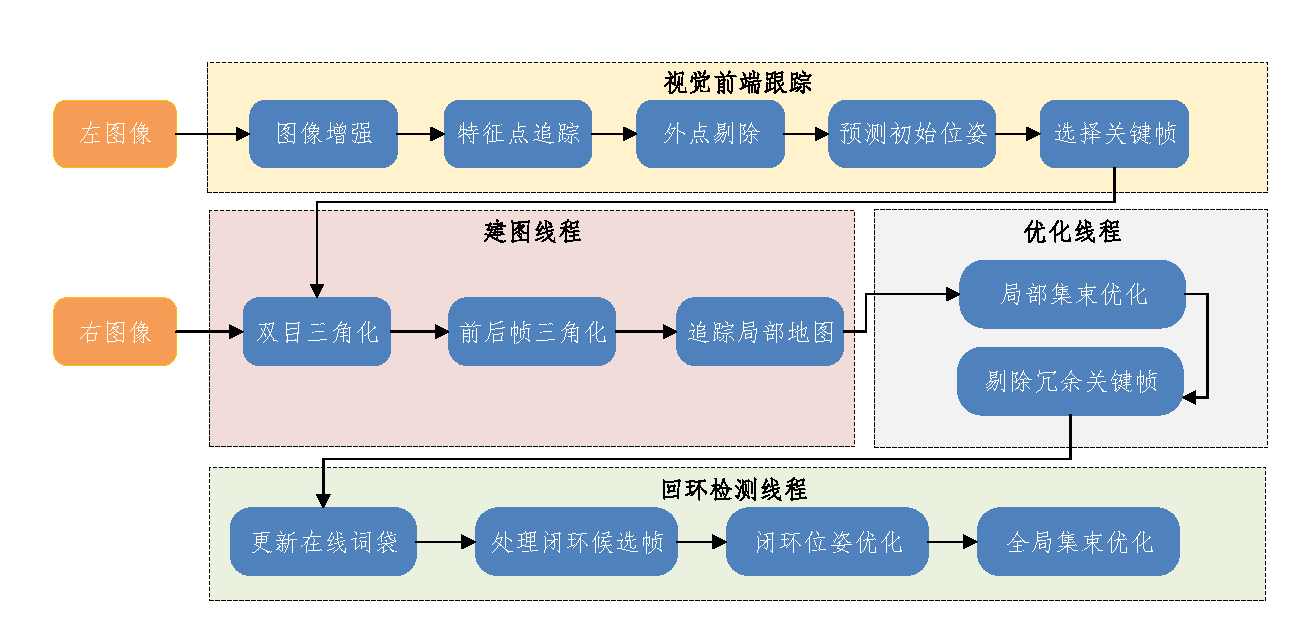
\includegraphics[width=14.5cm]{毕设图片/3-2-1}
%     \caption[OV2SLAM系统框架]{\label{fig:3-2}OV2SLAM系统框架\cite{OV2SLAM}}
% \end{figure}
% \section{传感器残差分析}
% 本章所提出的算法集成了双目相机、IMU和深度计三个传感器,如\autoref{fig:3-3}所示,
% 本节将介绍这些传感器获取信息的方式,并给出相应的优化处理方法。
% 本章节定义体坐标系为IMU坐标系,并定义${{\bf{T}}_{12}}$表示将从坐标系2变换到坐标系1的矩阵,$\bf{R}$表示旋转,
% $\bf{t}$表示平移,${c_1}{c_2}$分别代表左右相机的坐标系,b代表IMU和体坐标系,d代表深度计坐标系,w代表世界坐标系,
% ${{\bf{P}}_w}$表示三维点的坐标。
% \begin{figure}[htbp]
%     \centering
%     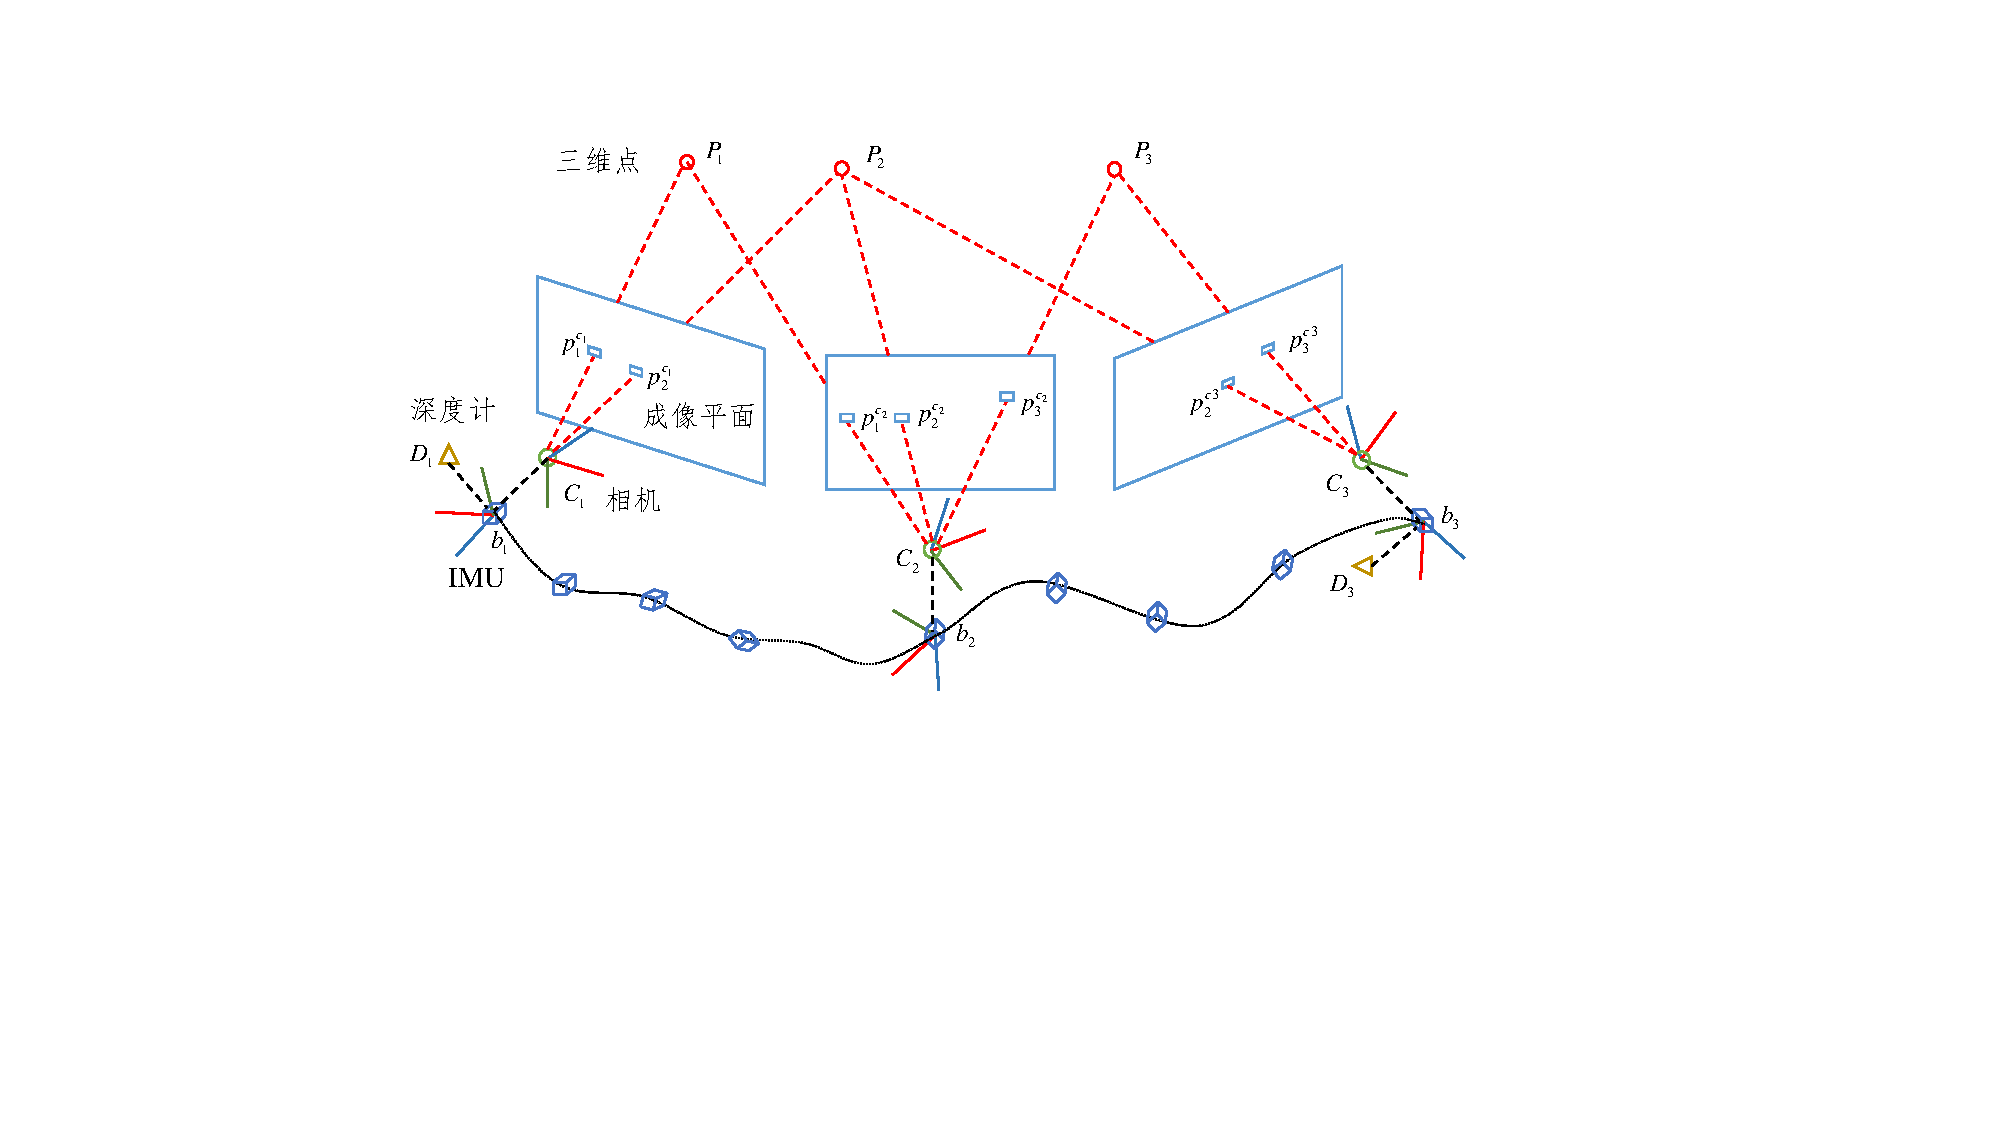
\includegraphics[width=14.5cm]{毕设图片/3-3.pdf}
%     \caption{\label{fig:3-3}RRVIP-SLAM“双目视觉-惯性-深度”感知示意图}
% \end{figure}

% \subsection{双目视觉重投影误差模型}
% 相机通过观测空间中的路标点计算位姿,相机由于制造误差会存在径向畸变和切向畸变,能用下式描述:
% \begin{equation}
%     \label{equ:3-1}
%     \left\{ {\begin{array}{*{20}{l}}
%         {{x_{{\rm{distort }}}} = x\left( {1 + {k_1}{r^2} + {k_2}{r^4} + {k_3}{r^6}} \right) + 2{p_1}xy + {p_2}\left( {{r^2} + 2{x^2}} \right)}\\
%         {{y_{{\rm{distort }}}} = y\left( {1 + {k_1}{r^2} + {k_2}{r^4} + {k_3}{r^6}} \right) + {p_1}\left( {{r^2} + 2{y^2}} \right) + 2{p_2}xy}
%         \end{array}} \right.
% \end{equation}
% 其中$k$和$p$均表示畸变参数,$x$和$y$表示像素坐标。
% 但在标定过程中能够计算出这些参数,并能对图像进行去畸变处理,本节考虑无畸变的针孔相机模型。相机针孔模型满足如下关系:
% \begin{equation}
%     \label{equ:3-2}
%     \left( {\begin{array}{*{20}{c}}
%         u\\
%         v\\
%         1
%         \end{array}} \right) = \frac{1}{Z}\left( {\begin{array}{*{20}{c}}
%         {{f_x}}&0&{{c_x}}\\
%         0&{{f_y}}&{{c_y}}\\
%         0&0&1
%         \end{array}} \right)\left[ {\begin{array}{*{20}{c}}
%         {\bf{R}}&{\bf{t}}\\
%         {{{\bf{0}}^{\bf{T}}}}&1
%         \end{array}} \right]\left( {\begin{array}{*{20}{c}}
%         {{x_w}}\\
%         {{y_w}}\\
%         {{z_w}}\\
%         1
%         \end{array}} \right) = \frac{1}{Z}{\bf{KT}}\left( {\begin{array}{*{20}{c}}
%         {{x_w}}\\
%         {{y_w}}\\
%         {{z_w}}\\
%         1
%         \end{array}} \right)
% \end{equation}

% 在SLAM位姿计算中,完成视觉初始化后,如\autoref{fig:3-3}所示,会使用地图中的路标点与当前图像中的特征点进行匹配,使用重投影误差进行优化。记地图中的路标点坐标为${{\bf{P}}_w} = {\bf{P'}} = {\left[ {\begin{array}{*{20}{c}}
%     {X'}&{Y'}&{Z'}
%     \end{array}} \right]^T}$,使用式 \eqref{equ:3-2}将这点投影到当前帧得到的像素点为${\bf{p'}} = {\left[ {\begin{array}{*{20}{c}}
%         {u'}&{v'}
%         \end{array}} \right]^T}$,通过特征点匹配对应这一帧的像素点为${\bf{p}} = {\left[ {\begin{array}{*{20}{c}}
%             u&v
%             \end{array}} \right]^T}$。

% 通常认为当匹配和重投影得到的像素点坐标误差最小时,估计出的位姿是最优解。那么将这么问题定义为一个最小二程问题,如式 \eqref{equ:3-3},本章使用李代数\cite{Lidai}$\xi $表示式 \eqref{equ:3-2}中的旋转${\bf{R}}$和平移${\bf{t}}$,这个过程中体坐标位姿和空间点坐标均可以优化。
% \begin{equation}
%     \label{equ:3-3}
%     \mathop {\min }\limits_\xi  \frac{1}{2}{r_c}({\bf{\xi }},{{\bf{P}}_w}){^2}
% \end{equation}
% 其中
% \begin{equation}
%     \label{equ:3-4}
%     {r_c}\left( \xi  \right) = \left( {u',v'} \right) - \left( {u,v} \right)
% \end{equation}

% 在实际应用中,均是优化体坐标系下的位姿${{\bf{T}}_{wb}}$,左相机的重投影坐标则表示为
% \begin{equation}
%     \label{equ:3-5}
%     p' = \frac{1}{Z}{\bf{K}}{{\bf{T}}_{c1b}}{{\bf{T}}_{bw}}{{\bf{P}}_w}
% \end{equation}

% 为了能在后续SLAM算法中使用列文伯格-马夸尔特优化算法 (L-M, Levenberg-Marquardt)算法\cite{LML,LMM}对重投影误差进行优化,计算重投影残差的雅可比矩阵,为了统一对位姿的更新方式,本文均使用右扰动对李代数进行更新。

% 首先,对体坐标系位姿进行求导,使用链式法则来表示:
% \begin{equation}
%     \label{equ:3-6}
%     \begin{aligned}
%         \mathbf{J}(\boldsymbol{\xi}) & =\frac{\partial r\left(\boldsymbol{\xi}, \mathbf{P}_{w}\right)}{\partial \boldsymbol{\xi}} \\
%         & =\frac{\partial r(\boldsymbol{\xi})}{\partial \mathbf{p}^{\prime}} \cdot \frac{\partial \mathbf{p}^{\prime}}{\partial \mathbf{p}_{\text {norm }}^{\prime}} \cdot \frac{\partial \mathbf{p}_{\text {norm }}^{\prime}}{\partial \mathbf{P}^{\prime}} \cdot \frac{\partial \mathbf{P}^{\prime}}{\partial \boldsymbol{\xi}} \\
%         & =\mathbf{J}_{0} \cdot \mathbf{J}_{1} \cdot \mathbf{J}_{2} \cdot \mathbf{J}_{3}
%         \end{aligned}
% \end{equation}
% 其中norm表示归一化向量
% \begin{equation}
%     \label{equ:3-7}
%     {\bf{p}}_{{\rm{norm }}}^\prime  = {\raise0.7ex\hbox{${{\bf{p'}}}$} \!\mathord{\left/
%  {\vphantom {{{\bf{p'}}} {Z'}}}\right.\kern-\nulldelimiterspace}
% \!\lower0.7ex\hbox{${Z'}$}}
% \end{equation}
% 由于误差函数式 \eqref{equ:3-3}是关于像素坐标的函数,所以对于一个特定的像素点${\bf{p}}$是关于${\bf{\xi }}$的常量,那么有:
% \begin{equation}
%     {{\bf{J}}_0} = \frac{{\partial {{\bf{p}} }}}{{\partial {{\bf{p}}^\prime }}} = {\bf{I}} \in {\mathbb{R}^{2 \times 2}}
% \end{equation}
% \begin{equation}
%     {{\bf{J}}_1} = \frac{{\partial {{\bf{p}}^\prime }}}{{\partial {\bf{p}}_{{\rm{norm }}}^\prime }} = \frac{{\partial (u,v)}}{{\partial \left( {X_{{\rm{norm }}}^\prime ,Y_{{\rm{norm }}}^\prime } \right)}}
% \end{equation}
% 由于${{\bf{p}}^\prime } = {\bf{K}} \cdot {\bf{p}}_{{\rm{norm }}}^\prime $,K的形式在式 \eqref{equ:2-1}已经给出,所以有:
% \begin{equation}
%     {{\bf{J}}_1} = \left[ {\begin{array}{*{20}{c}}
%         {{f_x}}&0\\
%         0&{{f_y}}
%         \end{array}} \right]
% \end{equation}
% \begin{equation}
%     {{\bf{J}}_2} = \frac{{\partial {\bf{p}}_{{\rm{norm }}}^\prime }}{{\partial {{\bf{P}}^\prime }}} = \frac{{\partial \left( {X_{{\rm{norm }}}^\prime ,Y_{{\rm{norm }}}^\prime } \right)}}{{\partial \left( {{X^\prime },{Y^\prime },{Z^\prime }} \right)}}
% \end{equation}
% 根据式 \eqref{equ:3-7}得
% \begin{equation}
%     {{\bf{J}}_2} = \left[ {\begin{array}{*{20}{c}}
%         {\frac{1}{{{Z^\prime }}}}&0&{ - \frac{{{X^\prime }}}{{{Z^{\prime 2}}}}}\\
%         0&{\frac{1}{{{Z^\prime }}}}&{ - \frac{{{Y^\prime }}}{{{Z^{\prime 2}}}}}
%         \end{array}} \right]
% \end{equation}
% 使用李代数模型${\bf{\xi }} = {\left[ {\begin{array}{*{20}{c}}
%     \rho &\phi 
%     \end{array}} \right]^T} \in {\mathbb{R}^6}$,与扰动模型$\delta {\bf{\xi }} = {\left[ {\begin{array}{*{20}{c}}
%         {\delta \rho }&{\delta \phi }
%         \end{array}} \right]^T}$求导:
% \begin{equation}
%     \begin{aligned}
%         {{\bf{J}}_3} & = \frac{{\partial {{\bf{P}}^\prime }}}{{\partial {\bf{\xi }}}}\\
%         & = \frac{{\partial ({{\bf{T}}_{c1b}}{\bf{T}}_{wb}^{ - 1}{\bf{P}})}}{{\partial {\bf{\xi }}}}\\
%         & = \frac{{\partial \left( {{{\bf{T}}_{c1b}}\left( {\exp {{\left( {{{\bf{\xi }}^ \wedge }} \right)}^{ - 1}}} \right){\bf{P}}} \right)}}{{\partial {\bf{\xi }}}}\\
%         & = \left[ {\begin{array}{*{20}{c}}
%         { - {{\bf{R}}_{c1w}}}&{{{\bf{R}}_{c1w}}{{\bf{R}}_{c1b}}{{\left( {{{\bf{R}}_{bw}}\left( {{\bf{P}} - {{\bf{t}}_{wb}}} \right)} \right)}^ \wedge }}
%         \end{array}} \right]
%     \end{aligned}
% \end{equation}
% 其中$^ \wedge$表示将向量转化为反对称矩阵。联立以上公式即可得到重投影误差关于体坐标系的雅克比矩阵。同样的方法能计算出空间点坐标的雅克比矩阵。
% \begin{equation}
%     \begin{aligned}
%         {\bf{J}}({{\bf{P}}_w}) & = \frac{{\partial r({\bf{\xi }},{{\bf{P}}_w})}}{{\partial {{\bf{P}}_w}}}\\
%         & = {{\bf{J}}_1}{{\bf{J}}_2}{{\bf{R}}_{c1w}}
%     \end{aligned}
% \end{equation}

% 对于右相机,重投影坐标能表示为
% \begin{equation}
%     p' = \frac{1}{Z}{\bf{K}}{{\bf{T}}_{c2b}}{{\bf{T}}_{bw}}{{\bf{P}}_w}
% \end{equation}
% 同样有
% \begin{equation}
%     \begin{aligned}
%         {{\bf{J}}_4} &= \frac{{\partial {{\bf{P}}^\prime }}}{{\partial {\bf{\xi }}}}\\
%             &= \frac{{\partial ({{\bf{T}}_{c2b}}{\bf{T}}_{wb}^{ - 1}{\bf{P}})}}{{\partial {\bf{\xi }}}}\\
%            & = \frac{{\partial \left( {{{\bf{T}}_{c2b}}\left( {\exp {{\left( {{{\bf{\xi }}^ \wedge }} \right)}^{ - 1}}} \right){\bf{P}}} \right)}}{{\partial {\bf{\xi }}}}\\
%           &  = \left[ {\begin{array}{*{20}{c}}
%         { - {{\bf{R}}_{c2w}}}&{{{\bf{R}}_{c2w}}{{\bf{R}}_{c2b}}{{\left( {{{\bf{R}}_{bw}}\left( {{\bf{P}} - {{\bf{t}}_{wb}}} \right)} \right)}^ \wedge }}
%         \end{array}} \right]
%     \end{aligned}
% \end{equation}
% 雅克比矩阵为
% \begin{equation}
%     \begin{aligned}
%         {\bf{J}}({\bf{\xi }})& = \frac{{\partial r({\bf{\xi }},{{\bf{P}}_w})}}{{\partial {\bf{\xi }}}}\\
%            & = {{\bf{J}}_0} \cdot {{\bf{J}}_1} \cdot {{\bf{J}}_2} \cdot {{\bf{J}}_4}
%     \end{aligned}
% \end{equation}

% \subsection{IMU预积分模型和残差模型}
% IMU通常内置了加速度计和陀螺仪,能够测量三个方向的加速度和三个方向的角速度。一般认为IMU测量的数据包括确定性误差bias和随机误差。随机误差满足高斯分布,也称为高斯噪声。

% 角速度测量的数学模型为:
% \begin{equation}
%     \begin{aligned}
%         {{\bf{\tilde \omega }}^b} = {{\bf{\omega }}^b} + {{\bf{b}}^g} + {{\bf{n}}^g}
%     \end{aligned}
% \end{equation}
% 其中${{\bf{\tilde \omega }}^b}$为体坐标系下的角速度测量值,${{\bf{\omega }}^b}$为角速度真值,${{\bf{b}}^g}$为角速度测量的bias,${{\bf{n}}^g}$为角速度测量的高斯噪声,满足${{\bf{n}}_g}\sim \eta \left( {{\bf{0}},\sigma _g^2 \cdot {{\bf{I}}_3}} \right)$。

% 加速度测量的数学模型为:
% \begin{equation}
%     {{\bf{\tilde a}}^b} = {{\bf{q}}_{bw}}\left( {{{\bf{a}}^w} + {{\bf{g}}^w}} \right) + {{\bf{b}}^a} + {{\bf{n}}^a}
% \end{equation}
% 其中${{\bf{\tilde a}}^b}$为体坐标系下的加速度测量值,${{\bf{a}}^w}$为世界坐标系下的加速度真值,${{\bf{g}}^w}$为世界坐标系下的重力加速度,${{\bf{b}}^a}$为加速度测量的bias,${{\bf{n}}^a}$为加速度测量的高斯噪声,满足${{\bf{n}}_a}\sim \eta \left( {{\bf{0}},\sigma _a^2 \cdot {{\bf{I}}_3}} \right)$。

% 在SLAM系统中,IMU的状态包括在世界坐标系下的坐标、速度、旋转、角速度和加速度的bias,记为:
% \begin{equation}
%     \label{equ:3-20}
%     x = \left[ {\begin{array}{*{20}{c}}
%         {{\bf{P}}_b^w}&{{\bf{q}}_b^w}&{\bf{v}}&{{{\bf{b}}^g}}&{{{\bf{b}}^a}}
%         \end{array}} \right]
% \end{equation}

% 对$i$时刻和$j$时刻之间IMU测量的加速度和角速度进行积分,能计算出系统的坐标、速度和旋转信息:
% \begin{equation}
%     \label{equ:3-21}
%     \begin{array}{l}
%         {{\bf{p}}_{w{b_j}}} = {{\bf{p}}_{w{b_i}}} + {\bf{v}}_i^w\Delta t + \iint_{{t \in [i,j]}}^{}{\left( {{{\bf{q}}_{w{b_t}}}{{\bf{a}}^{{b_t}}} - {{\bf{g}}^w}} \right)}\delta {t^2}\\
%         {\bf{v}}_j^w = {\bf{v}}_i^w + \int_{t \in [i,j]} {\left( {{{\bf{q}}_{w{b_t}}}{{\bf{a}}^{{b_t}}} - {{\bf{g}}^w}} \right)} \delta t\\
%         {{\bf{q}}_{w{b_j}}} = \int_{t \in [i,j]} {{{\bf{q}}_{w{b_t}}}}  \otimes \left[ {\begin{array}{*{20}{c}}
%         0\\
%         {\frac{1}{2}{{\bf{\omega }}^{{b_t}}}}
%         \end{array}} \right]\delta t
%         \end{array}
% \end{equation}
% 其中${\bf{q}}$表示四元数,${\bf{\omega }}$表示旋转角度。但这样会导致每次${{\bf{q}}_{wb}}$优化更新后,都需要重新进行积分,运算量非常大,因此本文使用IMU预积分\cite{预积分}模型,预积分模型仅仅跟IMU测量值有关,克服了重新积分的问题:
% \begin{equation}
%     \begin{array}{l}
%         {{\bf{p}}_{w{b_j}}} = {{\bf{p}}_{w{b_i}}} + {\bf{v}}_i^w\Delta t - \frac{1}{2}{{\bf{g}}^w}\Delta {t^2} + {{\bf{q}}_{w{b_i}}}\iint_{{t \in [i,j]}}^{}{\left( {{{\bf{q}}_{{b_i}{b_t}}}{{\bf{a}}^{{b_t}}}} \right)}\delta {t^2}\\
%         {\bf{v}}_j^w = {\bf{v}}_i^w - {{\bf{g}}^w}\Delta t + {{\bf{q}}_{w{b_i}}}\int_{t \in [i,j]} {\left( {{{\bf{q}}_{{b_i}{b_t}}}{{\bf{a}}^{{b_t}}}} \right)} \delta t\\
%         {{\bf{q}}_{w{b_j}}} = {{\bf{q}}_{w{b_i}}}\int_{t \in [i,j]} {{{\bf{q}}_{{b_i}{b_t}}}}  \otimes \left[ {\begin{array}{*{20}{c}}
%         0\\
%         {\frac{1}{2}{\omega ^{{b_t}}}}
%         \end{array}} \right]\delta t
%         \end{array}
% \end{equation}

% 定义位置、速度和角度的预积分量如下:
% \begin{equation}
%     \begin{array}{l}
%         {{\bf{\alpha }}_{{b_i}{b_j}}} = \iint_{{t \in [i,j]}}^{}{\left( {{{\bf{q}}_{{b_i}{b_t}}}{{\bf{a}}^{{b_t}}}} \right)}\delta {t^2}\\
%         {{\bf{\beta }}_{{b_i}{b_j}}} = \int_{t \in [i,j]} {\left( {{{\bf{q}}_{{b_i}{b_t}}}{{\bf{a}}^{{b_t}}}} \right)} \delta t\\
%         {{\bf{q}}_{{b_i}{b_j}}} = \int_{t \in [i,j]} {{{\bf{q}}_{{b_i}{b_t}}}}  \otimes \left[ {\begin{array}{*{20}{c}}
%         0\\
%         {\frac{1}{2}{{\bf{\omega }}^{{b_t}}}}
%         \end{array}} \right]\delta t
%         \end{array}
% \end{equation}
% 则IMU的状态量式 \eqref{equ:3-20}可以表示为:
% \begin{equation}
%     \left[ {\begin{array}{*{20}{c}}
%         {{{\bf{p}}_{w{b_j}}}}\\
%         {{\bf{v}}_j^w}\\
%         {{{\bf{q}}_{w{b_j}}}}\\
%         {{\bf{b}}_j^a}\\
%         {{\bf{b}}_j^g}
%         \end{array}} \right] = \left[ {\begin{array}{*{20}{c}}
%         {{{\bf{p}}_{w{b_i}}} + {\bf{v}}_i^w\Delta t - \frac{1}{2}{{\bf{g}}^w}\Delta {t^2} + {{\bf{q}}_{w{b_i}}}{\alpha _{{b_i}{b_j}}}}\\
%         {{\bf{v}}_i^w - {{\bf{g}}^w}\Delta t + {{\bf{q}}_{w{b_i}}}{{\bf{\beta }}_{{b_i}{b_j}}}}\\
%         {{{\bf{q}}_{w{b_i}}}{{\bf{q}}_{{b_i}{b_j}}}}\\
%         {{\bf{b}}_i^a}\\
%         {{\bf{b}}_i^g}
%         \end{array}} \right]
% \end{equation}

% IMU的残差定义为预积分的残差和bias的残差。预积分残差为用两时刻的状态构建与预积分量的差;bias的残差为两时刻的bias做差,因为一般认为IMU在短时间内的bias是固定的。所以IMU的残差定义如下:
% \begin{equation}
%     \label{equ:3-25}
%     {{\bf{r}}_{imu}} = \left[ {\begin{array}{*{20}{c}}
%         {{{\bf{r}}_p}}\\
%         {{{\bf{r}}_q}}\\
%         {{{\bf{r}}_v}}\\
%         {{{\bf{r}}_{ba}}}\\
%         {{{\bf{r}}_{bg}}}
%         \end{array}} \right] = \left[ {\begin{array}{*{20}{c}}
%         {{{\bf{q}}_{{b_i}w}}\left( {{{\bf{p}}_{w{b_j}}} - {{\bf{p}}_{w{b_i}}} - {\bf{v}}_i^w\Delta t + \frac{1}{2}{{\bf{g}}^w}\Delta {t^2}} \right) - {\alpha _{{b_i}{b_j}}}}\\
%         {2{{\left[ {{{\bf{q}}_{{b_j}{b_i}}} \otimes \left( {{{\bf{q}}_{{b_i}w}} \otimes {{\bf{q}}_{w{b_j}}}} \right)} \right]}_{xyz}}}\\
%         {{{\bf{q}}_{{b_i}w}}\left( {{\bf{v}}_j^w - {\bf{v}}_i^w + {{\bf{g}}^w}\Delta t} \right) - {{\bf{\beta }}_{{b_i}{b_j}}}}\\
%         {{\bf{b}}_j^a - {\bf{b}}_i^a}\\
%         {{\bf{b}}_j^g - {\bf{b}}_i^g}
%         \end{array}} \right]
% \end{equation}
% 为了能对IMU残差进行优化,需要计算残差的传递矩阵和雅可比矩阵,与视觉残差类似,使用右扰动对李代数进行更新。

% 在计算得到$k$时刻的误差后,由于噪声${{\bf{n}}^g}$和${{\bf{n}}^a}$的存在,使用基于泰勒展开的误差传递,从$k$时刻到$k+1$时刻的误差的传递由两部分组成:当前时刻的误差传递给下一时刻,当前时刻测量噪声传递给下一时刻。参考文献\cite{预积分}的公式,残差线性传递方程为:
% \begin{equation}
%     \left[ {\begin{array}{*{20}{c}}
%         {\delta {{\bf{\alpha }}_{{b_{k + 1}}b_{k + 1}^\prime }}}\\
%         {\delta {{\bf{q}}_{{b_{k + 1}}{b_{k + 1}}}}}\\
%         {\delta {{\bf{\beta }}_{{b_{k + 1}}b_{k + 1}^\prime }}}\\
%         {\delta {\bf{b}}_{k + 1}^a}\\
%         {\delta {\bf{b}}_{k + 1}^g}
%         \end{array}} \right] = {\bf{F}}\left[ {\begin{array}{*{20}{c}}
%         {\delta {{\bf{\alpha }}_{{b_k}b_k^\prime }}}\\
%         {\delta {{\bf{q}}_{{b_k}b_k^\prime }}}\\
%         {\delta {{\bf{\beta }}_{{b_k}b_k^\prime }}}\\
%         {\delta {\bf{b}}_k^a}\\
%         {\delta {\bf{b}}_k^g}
%         \end{array}} \right] + {\bf{G}}\left[ {\begin{array}{*{20}{c}}
%         {{\bf{n}}_k^a}\\
%         {{\bf{n}}_k^g}\\
%         {{\bf{n}}_{k + 1}^a}\\
%         {{\bf{n}}_{k + 1}^g}\\
%         {{{\bf{n}}_{{\bf{b}}_k^a}}}\\
%         {{{\bf{n}}_{{\bf{b}}_k^g}}}
%         \end{array}} \right]
% \end{equation}
% 其中F,G为两个时刻间的协方差传递方程:
% \begin{equation}
%     {\bf{F}} = \left[ {\begin{array}{*{20}{c}}
%         {\bf{I}}&{{{\bf{f}}_{12}}}&{{\bf{I}}\delta t}&{ - \frac{1}{4}\left( {{{\bf{q}}_{{b_i}{b_k}}} + {{\bf{q}}_{{b_i}{b_{k + 1}}}}} \right)\delta {t^2}}&{{{\bf{f}}_{15}}}\\
%         {\bf{0}}&{{\bf{I}} - {{[{\bf{\omega }}]}_ \times }}&{\bf{0}}&{\bf{0}}&{ - {\bf{I}}\delta t}\\
%         {\bf{0}}&{{{\bf{f}}_{32}}}&{\bf{I}}&{ - \frac{1}{2}\left( {{{\bf{q}}_{{b_i}{b_k}}} + {{\bf{q}}_{{b_i}{b_{k + 1}}}}} \right)\delta t}&{{{\bf{f}}_{35}}}\\
%         {\bf{0}}&{\bf{0}}&{\bf{0}}&{\bf{I}}&{\bf{0}}\\
%         {\bf{0}}&{\bf{0}}&{\bf{0}}&{\bf{0}}&{\bf{I}}
%         \end{array}} \right]
% \end{equation}
% \begin{equation}
%     {\bf{G}} = \left[ {\begin{array}{*{20}{c}}
%         {\frac{1}{4}{{\bf{q}}_{{b_i}{b_k}}}\delta {t^2}}&{{{\bf{g}}_{12}}}&{\frac{1}{4}{{\bf{q}}_{{b_i}{b_{k + 1}}}}\delta {t^2}}&{{{\bf{g}}_{14}}}&{\bf{0}}&{\bf{0}}\\
%         {\bf{0}}&{\frac{1}{2}{\bf{I}}\delta t}&{\bf{0}}&{\frac{1}{2}{\bf{I}}\delta t}&{\bf{0}}&{\bf{0}}\\
%         {\frac{1}{2}{{\bf{q}}_{{b_i}{b_k}}}\delta t}&{{{\bf{g}}_{32}}}&{\frac{1}{2}{{\bf{q}}_{{b_i}{b_{k + 1}}}}\delta t}&{{{\bf{g}}_{34}}}&{\bf{0}}&{\bf{0}}\\
%         {\bf{0}}&{\bf{0}}&{\bf{0}}&{\bf{0}}&{{\bf{I}}\delta t}&{\bf{0}}\\
%         {\bf{0}}&{\bf{0}}&{\bf{0}}&{\bf{0}}&{\bf{0}}&{{\bf{I}}\delta t}
%         \end{array}} \right]
% \end{equation}
% 其中的系数为:
% \begin{equation}
%     \begin{array}{l}
%         {{\bf{f}}_{12}} = \frac{{\partial {{\bf{\alpha }}_{{b_i}{b_{k + 1}}}}}}{{\partial \delta {{\bf{\theta }}_{{b_k}b_k^\prime }}}} =  - \frac{1}{4}\left( {{{\bf{R}}_{{b_i}{b_k}}}{{\left[ {{{\bf{a}}^{{b_k}}} - {\bf{b}}_k^a} \right]}_ \times }\delta {t^2} + {{\bf{R}}_{{b_i}{b_{k + 1}}}}{{\left[ {\left( {{{\bf{a}}^{{b_{k + 1}}}} - {\bf{b}}_k^a} \right)} \right]}_ \times }\left( {{\bf{I}} - {{[{\bf{\omega }}]}_ \times }\delta t} \right)\delta {t^2}} \right)\\
%         {{\bf{f}}_{32}} = \frac{{\partial {{\bf{\beta }}_{{b_i}{b_{k + 1}}}}}}{{\partial \delta {{\bf{\theta }}_{{b_k}b_k^\prime }}}} =  - \frac{1}{2}\left( {{{\bf{R}}_{{b_i}{b_k}}}{{\left[ {{{\bf{a}}^{{b_k}}} - {\bf{b}}_k^a} \right]}_ \times }\delta t + {{\bf{R}}_{{b_i}{b_{k + 1}}}}{{\left[ {\left( {{{\bf{a}}^{{b_{k + 1}}}} - {\bf{b}}_k^a} \right)} \right]}_ \times }\left( {{\bf{I}} - {{[{\bf{\omega }}]}_ \times }\delta t} \right)\delta t} \right)\\
%         {{\bf{f}}_{15}} = \frac{{\partial {{\bf{\alpha }}_{{b_i}{b_{k + 1}}}}}}{{\partial \delta {\bf{b}}_k^g}} =  - \frac{1}{4}\left( {{{\bf{R}}_{{b_i}{b_{k + 1}}}}{{\left[ {\left( {{{\bf{a}}^{{b_{k + 1}}}} - {\bf{b}}_k^a} \right)} \right]}_ \times }\delta {t^2}} \right)( - \delta t)\\
%         {{\bf{f}}_{35}} = \frac{{\partial {\beta _{{b_i}{b_{k + 1}}}}}}{{\partial \delta {\bf{b}}_k^g}} =  - \frac{1}{2}\left( {{{\bf{R}}_{{b_i}{b_{k + 1}}}}{{\left[ {\left( {{{\bf{a}}^{{b_{k + 1}}}} - {\bf{b}}_k^a} \right)} \right]}_ \times }\delta t} \right)( - \delta t)\\
%         {{\bf{g}}_{12}} = \frac{{\partial {{\bf{\alpha }}_{{b_i}{b_{k + 1}}}}}}{{\partial {\bf{n}}_k^g}} = {{\bf{g}}_{14}} = \frac{{\partial {{\bf{\alpha }}_{{b_i}{b_{k + 1}}}}}}{{\partial {\bf{n}}_{k + 1}^g}} =  - \frac{1}{4}\left( {{{\bf{R}}_{{b_i}{b_{k + 1}}}}{{\left[ {\left( {{{\bf{a}}^{{b_{k + 1}}}} - {\bf{b}}_k^a} \right)} \right]}_ \times }\delta {t^2}} \right)\left( {\frac{1}{2}\delta t} \right)\\
%         {{\bf{g}}_{32}} = \frac{{\partial {{\bf{\beta }}_{{b_i}{b_{k + 1}}}}}}{{\partial {\bf{n}}_k^g}} = {{\bf{g}}_{34}} = \frac{{\partial {{\bf{\beta }}_{{b_i}{b_{k + 1}}}}}}{{\partial {\bf{n}}_{k + 1}^g}} =  - \frac{1}{2}\left( {{{\bf{R}}_{{b_i}{b_{k + 1}}}}{{\left[ {\left( {{{\bf{a}}^{{b_{k + 1}}}} - {\bf{b}}_k^a} \right)} \right]}_ \times }\delta {t^2}} \right)\left( {\frac{1}{2}\delta t} \right)
%         \end{array}
% \end{equation}

% 在SLAM位姿优化中,通常使用两个相机关键帧之间的IMU预积分对位姿进行优化,所以有以下待优化变量:
% \begin{equation}
%     \left[ {{{\bf{p}}_{w{b_k}}},{{\bf{q}}_{w{b_k}}},{\bf{v}}_k^w,{\bf{b}}_k^a,{\bf{b}}_k^g,{{\bf{p}}_{w{b_{k + 1}}}},{{\bf{q}}_{w{b_{k + 1}}}},{\bf{v}}_{k + 1}^w,{\bf{b}}_{k + 1}^a,{\bf{b}}_{k + 1}^g} \right]
% \end{equation}
% 将其分组,便于后续在SLAM算法中使用L-M算法\cite{LML,LMM}后续求导:
% \begin{equation}
%     \begin{array}{l}
%         {r_0} = \left[ {\begin{array}{*{20}{c}}
%         {{{\bf{p}}_{w{b_k}}}}&{{{\bf{q}}_{w{b_k}}}}
%         \end{array}} \right]\\
%         {r_1} = \left[ {\begin{array}{*{20}{c}}
%         {{\bf{v}}_k^w}&{{\bf{b}}_k^a}&{{\bf{b}}_k^g}
%         \end{array}} \right]\\
%         {r_2} = \left[ {\begin{array}{*{20}{c}}
%         {{{\bf{p}}_{w{b_{k + 1}}}}}&{{{\bf{q}}_{w{b_{k + 1}}}}}
%         \end{array}} \right]\\
%         {r_3} = \left[ {\begin{array}{*{20}{c}}
%         {{\bf{v}}_{k + 1}^w}&{{\bf{b}}_{k + 1}^a}&{{\bf{b}}_{k + 1}^g}
%         \end{array}} \right]
%         \end{array}
% \end{equation}
% 则残差r相对于以上变量的雅克比矩阵可以表示为:
% \begin{equation}
%     \label{equ:3-32}
%     \begin{aligned}
%         {\bf{J}}{[0]^{15 \times 7}} 
%         & = \left[ {{\frac{{\partial {\bf{r}}}}{{\partial {{\bf{p}}_{w{b_k}}}}}}, {\frac{{\partial {\bf{r}}}}{{\partial {{\bf{q}}_{w{b_k}}}}}}} \right] \\
%         & = \left[ {\begin{array}{*{20}{c}}
%         { - {{\bf{q}}_{{b_k}w}}}&{{{\left[ {{{\bf{q}}_{{b_k}w}}\left( {{{\bf{p}}_{w{b_{k + 1}}}} - {{\bf{p}}_{w{b_k}}} - {\bf{v}}_k^w\delta t + \frac{1}{2}{{\bf{g}}^w}\delta {t^2}} \right)} \right]}^ \wedge }}\\
%         {\bf{0}}&{ - \left[ {{{\bf{q}}_{{b_{k + 1}}w}} \otimes {{\bf{q}}_{w{b_k}}}} \right] \otimes {{\bf{q}}_{{b_k}{b_{k + 1}}}}}\\
%         {\bf{0}}&{{{\left[ {{{\bf{q}}_{{b_k}w}}\left( {{\bf{v}}_{k + 1}^w - {\bf{v}}_k^w + {{\bf{g}}^w}\delta t} \right)} \right]}^ \wedge }}\\
%         {\bf{0}}&{\bf{0}}\\
%         {\bf{0}}&{\bf{0}}
%         \end{array}} \right]
%     \end{aligned}
% \end{equation}

% \begin{equation}
%     \label{equ:3-33}
%     \begin{aligned}
%         {\bf{J}}{[1]^{15 \times 9}} & = \left[ {\frac{{\partial {\bf{r}}}}{{\partial {\bf{v}}_k^w}},\frac{{\partial {\bf{r}}}}{{\partial {\bf{b}}_k^a}},\frac{{\partial {\bf{r}}}}{{\partial {\bf{b}}_k^g}}} \right] \\
%         & = \left[ {\begin{array}{*{20}{c}}
%         { - {{\bf{q}}_{{b_k}w}}\delta t}&{\frac{1}{4}\left( {{{\bf{q}}_{{b_i}{b_k}}} + {{\bf{q}}_{{b_i}{b_{k + 1}}}}} \right)\delta {t^2}}&{ - {{\bf{f}}_{15}}}\\
%         {\bf{0}}&{\bf{0}}&{\left[ {{{\bf{q}}_{{b_{k + 1}}w}} \otimes {{\bf{q}}_{w{b_k}}} \otimes {{\bf{q}}_{{b_k}{b_{k + 1}}}}} \right]\delta t}\\
%         { - {{\bf{q}}_{{b_k}w}}}&{\frac{1}{2}\left( {{{\bf{q}}_{{b_i}{b_k}}} + {{\bf{q}}_{{b_i}{b_{k + 1}}}}} \right)\delta t}&{ - {{\bf{f}}_{35}}}\\
%         {\bf{0}}&{ - I}&{\bf{0}}\\
%         {\bf{0}}&{\bf{0}}&{ - I}
%         \end{array}} \right]
%     \end{aligned}
% \end{equation}
% \begin{equation}
%     \label{equ:3-34}
%     {\bf{J}}{[2]^{15 \times 9}} = \left[ {\frac{{\partial {\bf{r}}}}{{\partial {{\bf{p}}_{w{b_{k + 1}}}}}},\frac{{\partial {\bf{r}}}}{{\partial {{\bf{q}}_{w{b_{k + 1}}}}}}} \right] = \left[ {\begin{array}{*{20}{c}}
%         {{{\bf{q}}_{{b_k}w}}}&{\bf{0}}\\
%         {\bf{0}}&{{{\bf{q}}_{{b_{k{\rm{ + }}1}}{b_k}}} \otimes {{\bf{q}}_{{b_k}w}} \otimes {{\bf{q}}_{w{b_{k + 1}}}}}\\
%         {\bf{0}}&{\bf{0}}\\
%         {\bf{0}}&{\bf{0}}\\
%         {\bf{0}}&{\bf{0}}
%         \end{array}} \right]
% \end{equation}
% \begin{equation}
%     \label{equ:3-35}
%     {\bf{J}}{[3]^{15 \times 9}} = \left[ {\frac{{\partial {\bf{r}}}}{{\partial {\bf{v}}_{k + 1}^w}},\frac{{\partial {\bf{r}}}}{{\partial {\bf{b}}_{k + 1}^a}},\frac{{\partial {\bf{r}}}}{{\partial {\bf{b}}_{k + 1}^g}}} \right] = \left[ {\begin{array}{*{20}{c}}
%         {\bf{0}}&{\bf{0}}&{\bf{0}}\\
%         {\bf{0}}&{\bf{0}}&{\bf{0}}\\
%         {{{\bf{q}}_{{b_k}w}}}&{\bf{0}}&{\bf{0}}\\
%         {\bf{0}}&{\bf{I}}&{\bf{0}}\\
%         {\bf{0}}&{\bf{0}}&{\bf{I}}
%         \end{array}} \right]
% \end{equation}

% \subsection{深度传感器的误差模型}
% 深度传感器能够测量水下的压强,并通过水的密度计算所处位置在水下的深度。由于水的压强在各个方向都是相等的,因此深度计的外部参数仅需考虑平移${{\bf{t}}_{db}}$,不需要考虑旋转。但在使用时,并不能确定深度计在系统初始化时的值${d_0}$,将在后续的优化中对这个参数进行估计。

% 深度计残差为使用深度计测量的高度变化值与体坐标系的z坐标差,用方程表示为:
% \begin{equation}
%     \label{equ:3-36}
%     {r_d}\left( {{\bf{\xi }},{d_0}} \right) = d - {d_0} - {\bf{e}} \cdot \left( {{{\bf{T}}_{wb}}{{\bf{t}}_{bd}}} \right)
% \end{equation}
% 其中
% \begin{equation}
%     {\bf{e}} = \left[ {\begin{array}{*{20}{c}}
%         0&0&1
%         \end{array}} \right]
% \end{equation}

% 为了能在后续SLAM算法中使用L-M算法对深度计数据优化,计算上述方程与体坐标系位姿的雅克比矩阵:
% \begin{equation}
%     \begin{aligned}
%         {\bf{J}}({\bf{\xi }},{d_0}) &= \frac{{\partial r({\bf{\xi }},{d_0})}}{{\partial {\bf{\xi }}}}\\
%          &= \left[ {\begin{array}{*{20}{c}}
%         { - {\bf{e}}}&{ - {\bf{e}} \cdot {{\bf{R}}_{wb}} \cdot {\bf{t}}_{bd}^ \wedge }
%         \end{array}} \right]
%     \end{aligned}
% \end{equation}
% 在初始化过程中对初始深度${d_0}$的雅克比矩阵为:
% \begin{equation}
%     \begin{aligned}
%             {\bf{J}}({\bf{\xi }},{d_0}) &= \frac{{\partial r({\bf{\xi }},{d_0})}}{{\partial {d_0}}}\\
%             & =  - 1
%     \end{aligned}
% \end{equation}

% \section{“双目视觉-惯性-深度”多传感器融合}
% 为了在水下环境中稳定运行,如\autoref{fig:3-3}所示,RRVIP-SLAM融合了IMU和深度计传感器,三维地图点投影到相机平面上,IMU在两个相机帧之间计算预积分,深度计输出到水面的深度信息。本节将介绍三种传感器时间同步优化融合方法与具体算法的实现。

% \subsection{“双目视觉-惯性-深度”联合初始化}

% 由于双目视觉系统能直接计算三维点坐标,所以视觉初始化在特征点数量足够时即可认为完成。对于惯性和深度传感器,在初始化阶段,认为双目视觉计算的位姿是准确的,通过构造IMU和深度计初始得到的位姿和视觉得到的位姿的残差方程,并使用最小二乘优化方法进行求解。使用滑动窗口法,从视觉前端选取关键帧,计算连续关键帧之间的IMU的预积分,并通过时间关系找到每一个深度计数据对应的关键帧,当关键帧有10帧时,启动联合初始化优化。

% \begin{figure}[H]
%     \centering
%     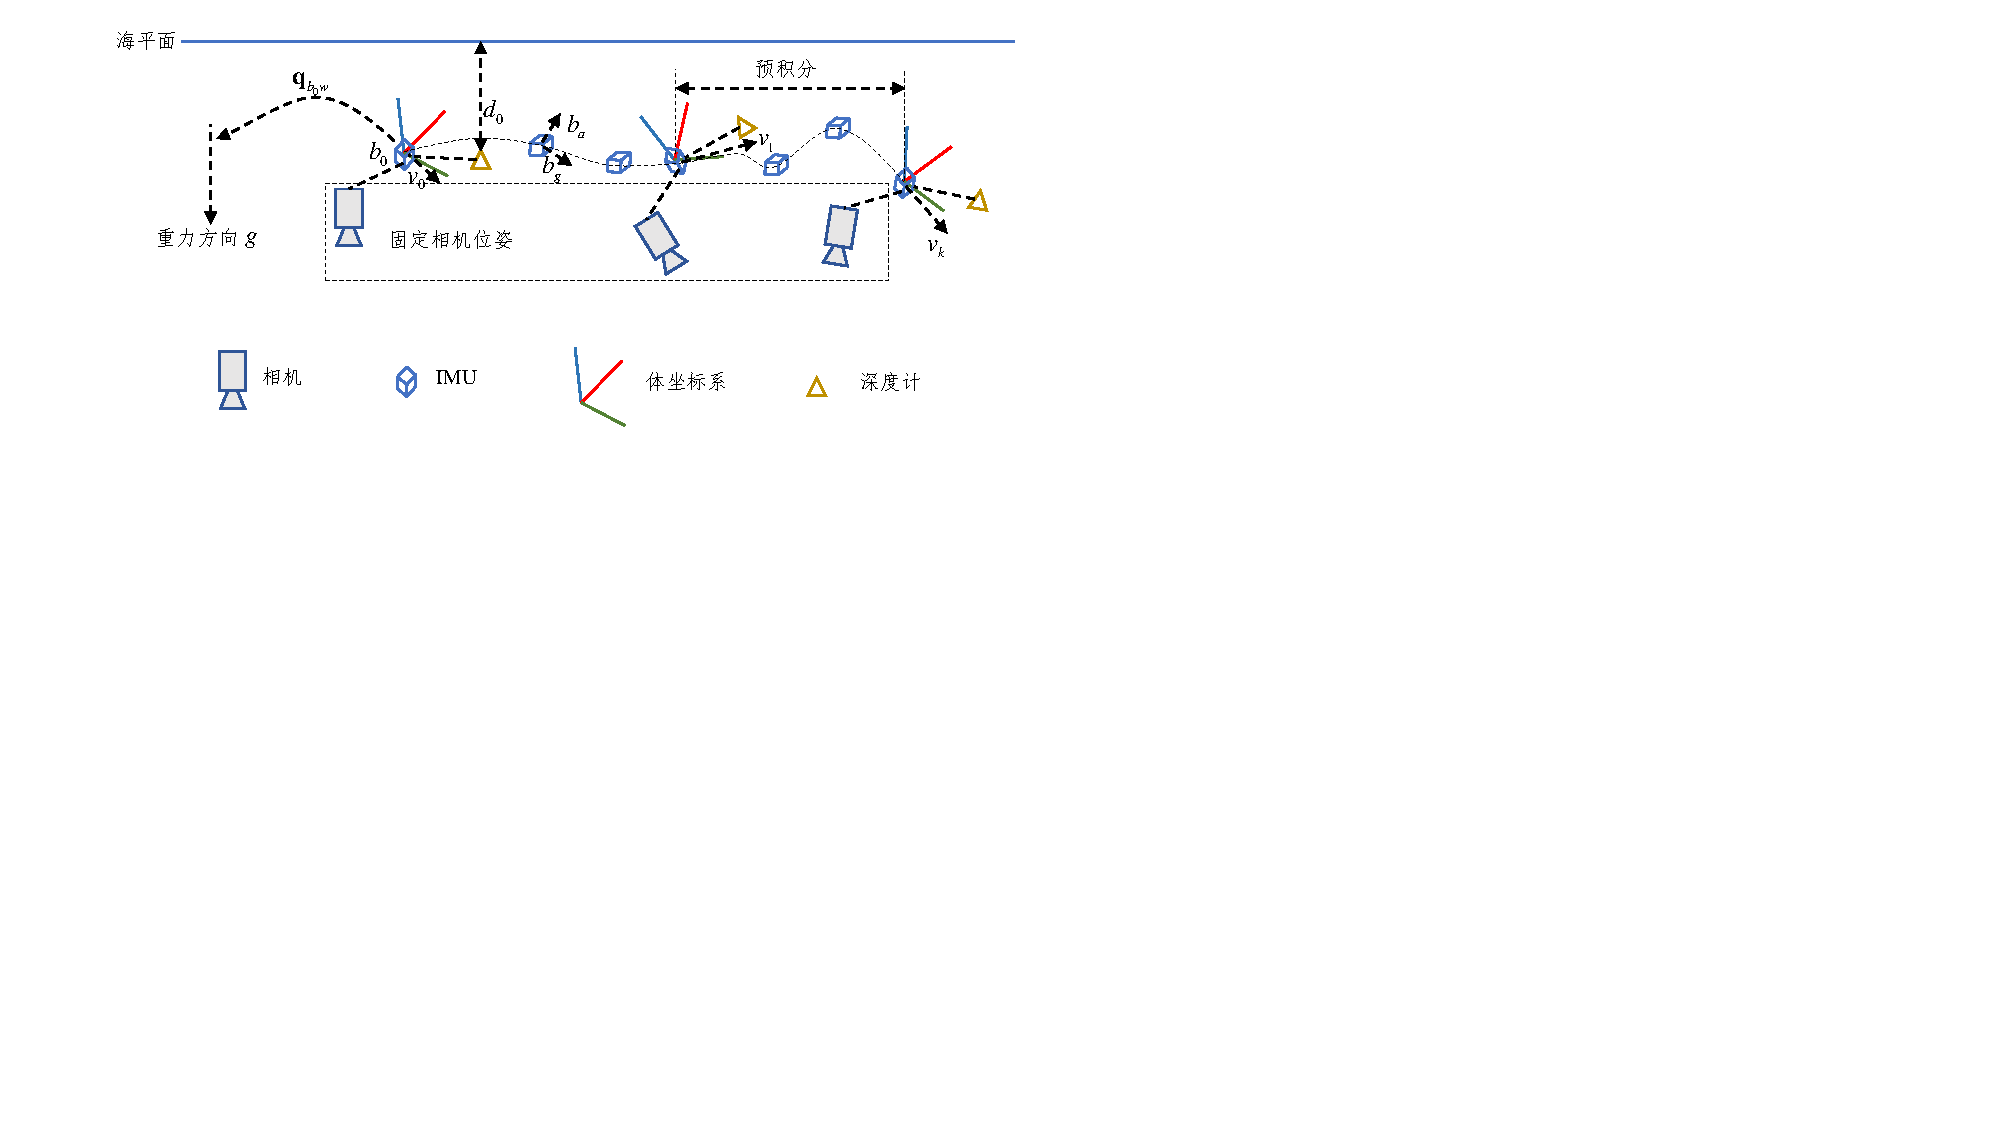
\includegraphics[width=14.5cm]{毕设图片/3-4.pdf}
%     \caption{\label{fig:3-4}RRVIP-SLAM初始化示意图}
% \end{figure}

% 本节采用最大后验分布方法来解算该初始化问题,如\autoref{fig:3-4}所示,需要求解的参数为系统尺度${s}$、第一个关键帧的体坐标系${b_0}$相对于重力方向的旋转${{\bf{q}}_{{b_0}w}}$、IMU加速度和角速度的零点偏移${b_a}$和${b_g}$、第一个关键帧的的体坐标系距离水平面的垂直距离${d_0}$、每个关键帧时刻下的体坐标系速度${v_k}$,记${v_{0:k}}$为用于初始化的所有关键帧对应的速度。由于本文所研究的双目视觉系统能计算绝对位姿,所以将系统尺度定义为$s = 1$,那么要求解的状态可以表示为:
% \begin{equation}
%     \label{equ:3-40}
%     x = \left\{ {\begin{array}{*{20}{c}}
%         {{{\bf{q}}_{{b_0}w}}}&{{b_a}}&{{b_g}}&{{d_0}}&{{v_{0:k}}}
%         \end{array}} \right\}
% \end{equation}

% 如\autoref{fig:3-4}所示,在求解过程中固定相机位姿,并构建关于式 \eqref{equ:3-25}中${{\bf{r}}_{imu}}$和式 \eqref{equ:3-36}中${{\bf{r}}_d}$的最小二程函数:
% \begin{equation}
%     \label{equ:3-41}
%     {\chi _{init}} = \arg \min \sum\limits_{i = 0}^k {\left( {{{\left\| {e_{imu}^i} \right\|}^2} + {{\left\| {e_p^i} \right\|}^2}} \right)} 
% \end{equation}
% 使用L-M方法对式 \eqref{equ:3-41}进行优化,并通过3.3节中推导的雅克比公式 (\ref{equ:3-32})--(\ref{equ:3-35})
% 计算梯度,计算得到目标函数式 \eqref{equ:3-41}值最小时的系统状态下的式 \eqref{equ:3-40}。

% \subsection{“双目视觉-惯性-深度”联合位姿计算}
% 为了提高系统的鲁棒性,本算法前端的流程为当系统刚完成初始化或者重定位时,采用Lucas Kanade (LK)光流法\cite{LK}对特征点进行匹配,再使用PnP (Perspective-n-Point)算法计算初始位姿;正常跟踪时,会使用当前帧与上一帧之间的IMU数据进行积分预测当前帧的位姿;最后使用三种传感器对系统状态进行紧耦合优化。
% \subsubsection{光流法特征点匹配}
% 光流法用于寻找前一帧图像中的特征点在当前帧对应的像素点坐标,光流是空间运动物体在相机成像面上的像素运动的瞬时速度,LK光流是SLAM中最常用的方法。该算法基于以下三个假设:

% (1)光度一致性:认为目标点从不同角度观测到的像素值是一致的。

% (2)时间持续性:认为相机图像每两帧之间运动很小,像素位置变化很小。

% (3)空间一致性:认为图像中的子窗口有相似的运动。
% % \begin{itemize}
% %     \item{光度一致性:认为目标点从不同角度观测到的像素值是一致的。}
% %     \item{时间持续性:认为相机图像每两帧之间的运动很小,像素位置不会变化很大。}
% %     \item{空间一致性:认为图像中的子窗口有相似的运动。}
% % \end{itemize}

% \begin{figure}[htbp]
%     \centering
%     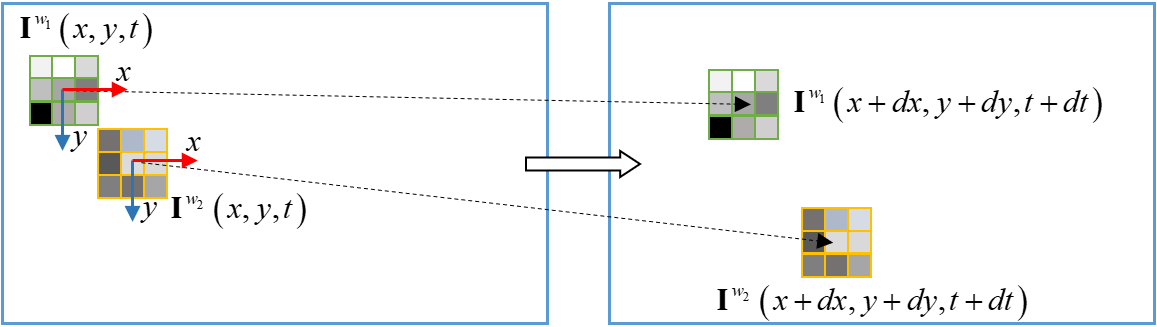
\includegraphics[width=14.5cm]{毕设图片/3-5}
%     \caption{\label{fig:3-5}光流法原理图}
% \end{figure}
% 如\autoref{fig:3-5}所示,当窗口${w_1}$中存在已经提取到特征点时,使用光流法寻找右图中的对应点,LK光流法将图像划分为很多个大小为$m \times m$的小窗口如${w_1}$和${w_2}$,它含有${m^2}$数量的像素,计算出窗口中每一个点在运动后对应的点的像素坐标。根据上述假设光度一致性假设有:
% \begin{equation}
%     {{\bf{I}}^w}\left( {x,y,t} \right) = {{\bf{I}}^w}\left( {x + dx,y + dy,t + dt} \right)
% \end{equation}
% 对右边进行泰勒展开,并保留一阶项:
% \begin{equation}
%     {{\bf{I}}^w}(x + {\rm{d}}x,y + {\rm{d}}y,t + {\rm{d}}t) \approx {{\bf{I}}^w}(x,y,t) + \frac{{\partial {\bf{I}}}}{{\partial x}}{\rm{d}}x + \frac{{\partial {\bf{I}}}}{{\partial y}}{\rm{d}}y + \frac{{\partial {\bf{I}}}}{{\partial t}}{\rm{d}}t
% \end{equation}
% 而假设了光度不会变,所以有:
% \begin{equation}
%     \begin{array}{c}
%         \frac{{\partial {\bf{I}}}}{{\partial x}}{\rm{d}}x + \frac{{\partial {\bf{I}}}}{{\partial y}}{\rm{d}}y + \frac{{\partial {\bf{I}}}}{{\partial t}}{\rm{d}}t = 0\\
%         \frac{{\partial {\bf{I}}}}{{\partial x}}\frac{{{\rm{d}}x}}{{\;{\rm{d}}t}} + \frac{{\partial {\bf{I}}}}{{\partial y}}\frac{{{\rm{d}}y}}{{dt}} =  - \frac{{\partial {\bf{I}}}}{{\partial t}}
%         \end{array}
% \end{equation}

% 根据上述空间一致性假设:认为该窗口内像素具有相同的运动,因此对这个小窗口共有${m^2}$个方程。记$x$方向的梯度为${\nabla _x} = {{\partial I} \mathord{\left/
% {\vphantom {{\partial I} {\partial x}}} \right.
% \kern-\nulldelimiterspace} {\partial x}}$,y方向的梯度为${\nabla _y} = {{\partial I} \mathord{\left/
% {\vphantom {{\partial I} {\partial y}}} \right.
% \kern-\nulldelimiterspace} {\partial y}}$,时间t的梯度为${\nabla _t} = {{\partial I} \mathord{\left/
% {\vphantom {{\partial I} {\partial t}}} \right.
% \kern-\nulldelimiterspace} {\partial t}}$,图像中$x$方向的位移为$u$,$y$方向的位移为$v$,那么有:
% \begin{equation}
%     {\left[ {\begin{array}{*{20}{c}}
%         {{\nabla _x}}&{{\nabla _y}}
%         \end{array}} \right]_k}\left[ {\begin{array}{*{20}{c}}
%         u\\
%         v
%         \end{array}} \right] =  - {{\bf{I}}_{tk}},k = 1,2, \ldots ,{m^2}
% \end{equation}
% 该方程的最小二乘解为:
% \begin{equation}
%     {\left[ {\begin{array}{*{20}{l}}
%         u\\
%         v
%         \end{array}} \right]^*} =  - {\left( {{{\bf{A}}^{\rm{T}}}{\bf{A}}} \right)^{ - 1}}{{\bf{A}}^{\rm{T}}}{\bf{b}}
% \end{equation}
% 其中
% \begin{equation}
%     {\bf{A}} = \left[ {\begin{array}{*{20}{c}}
%         {{{\left[ {{{\bf{I}}_x},{{\bf{I}}_y}} \right]}_1}}\\
%          \vdots \\
%         {{{\left[ {{{\bf{I}}_x},{{\bf{I}}_y}} \right]}_k}}
%         \end{array}} \right],{\bf{b}} = \left[ {\begin{array}{*{20}{c}}
%         {{{\bf{I}}_{t1}}}\\
%          \vdots \\
%         {{{\bf{I}}_{tk}}}
%         \end{array}} \right]
% \end{equation}

% \subsubsection{PnP算法求解初始位姿}
% 使用光流法匹配完成当前帧和上一帧的特征点,如\autoref{fig:3-6}所示,上一帧的特征点${p_1}$对应的地图点$P$是已知的,那么就转换成了一个已知地图中3D点$P$坐标和当前帧对应的像素点坐标${p_2}$,所以可以使用PnP算法求解当前帧的位姿。
% \begin{figure}[htbp]
%     \centering
%     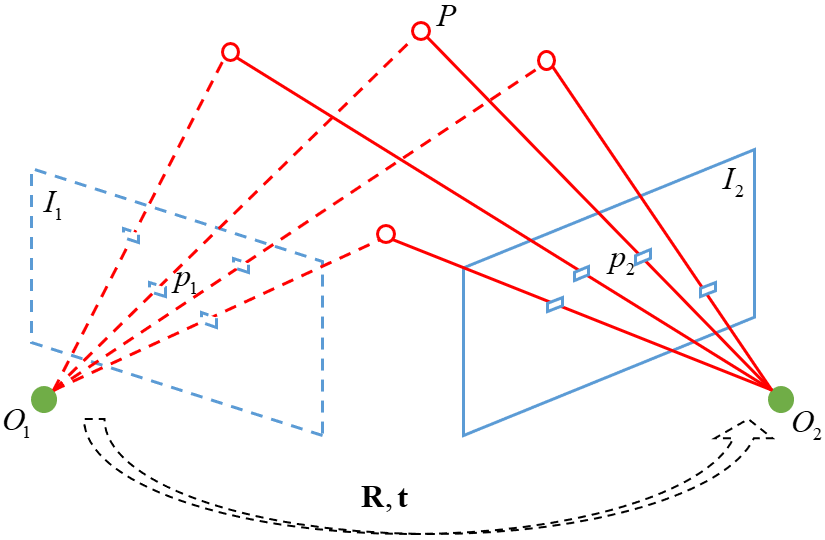
\includegraphics[width=10cm]{毕设图片/3-6}
%     \caption{\label{fig:3-6}PnP算法图解}
% \end{figure}

% 本文在SLAM系统中使用恒速模型与非线性优化的方式计算这个过程。恒速模型是认为短时间内系统的运动速度是恒定的,所以上一帧的位姿${{\bf{T}}_{w{b_1}}}$和上上帧位姿${{\bf{T}}_{w{b_2}}}$的相对位姿近似等于这一帧位姿${{\bf{T}}_{w{b_3}}}$相对于上一帧的位姿,即:
% \begin{equation}
%     {{\bf{T}}_{{b_2}{b_1}}} \simeq {{\bf{T}}_{{b_3}{b_2}}}
% \end{equation}
% 用${{\bf{T}}_{{b_2}{b_1}}}$作为PnP算法的初始解,然后使用非线性优化的方式优化3.3节中介绍的重投影误差,本文使用ceres库对3.3.1节中的式 \eqref{equ:3-3}进行优化。

% \subsubsection{IMU位姿预测初始位姿}
% 在系统跟踪状态正常时,使用上一帧的位姿与当前帧和上一帧之间的IMU积分计算出这一帧的初始位姿。预测的过程中不需要进行优化,所以采用IMU传统的积分方式进行计算,采用3.3.2节中的式 \eqref{equ:3-21}计算。

% \subsubsection{紧耦合优化}

% 在计算得到初始位置后,使用L-M优化方法对视觉、IMU、深度传感器进行BA紧耦合优化,如\autoref{fig:3-7}所示。

% \begin{figure}[H]
%     \centering
%     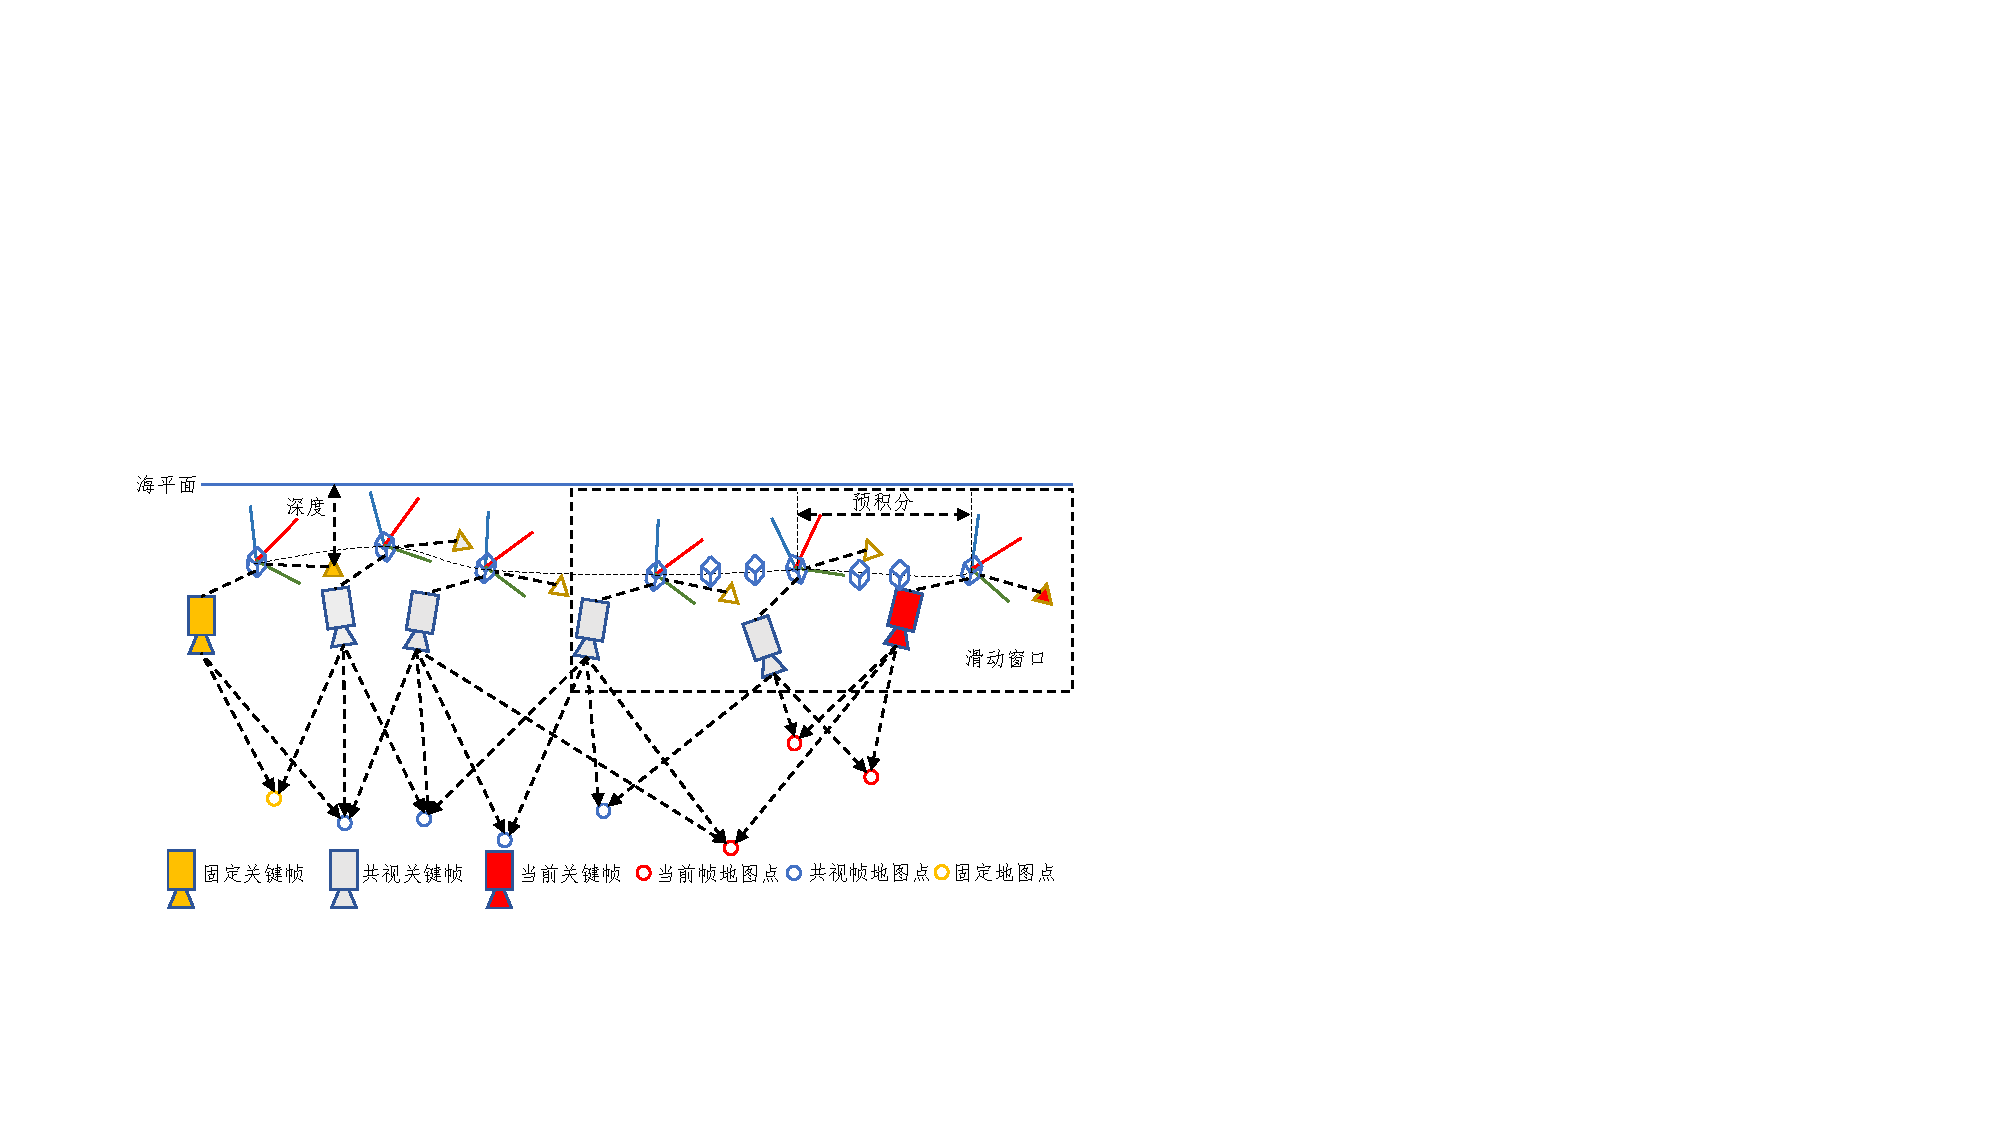
\includegraphics[width=14.5cm]{毕设图片/3-7.pdf}
%     \caption{\label{fig:3-7}紧耦合局部BA优化}
% \end{figure}

% 视觉部分紧耦合优化的策略如下:首先将所有能看到当前关键帧的特征点的关键帧定为共视帧;然后将能看到共视帧的地图点但不属于共视帧的帧设为固定关键帧,用作优化的约束;当前帧和共视帧的地图点中不属于固定关键帧的点三维坐标也加入优化目标;固定帧的地图点设置为优化的约束。
% IMU部分紧耦合优化的策略如下:使用滑动窗口的方法对IMU残差进行优化,以时间先后的关系选择与当前帧最接近的10帧,计算这10帧中每2帧之间的IMU残差。
% 深度计部分紧耦合优化策略为,计算当前测量的深度与初始深度的差,通过3.3节中介绍的公式计算残差并进行优化。
% 最后,将三个传感器融合,构建关于式 \eqref{equ:3-4}中${{\bf{r}}_{imu}}$、式 \eqref{equ:3-25}中${{\bf{r}}_d}$和式 \eqref{equ:3-36}中${{\bf{r}}_c}$的最小二程函数:
% \begin{equation}
%     {\chi} = \arg \min \sum\limits_{i = 0}^k {\left( {{{\left\| {e_{imu}^i} \right\|}^2} + {{\left\| {e_p^i} \right\|}^2} + {{\left\| {e_c^i} \right\|}^2}} \right)} 
% \end{equation}
% 后续将3.3节中介绍的残差计算公式和雅克比矩阵代入L-M算法进行优化,本文使用Ceres库对其优化。

% \section{数据集试验}
% 完成上述算法设计和C++ 部署后,本文在公开实测数据集上测试所提出的RRVIP-SLAM 算法性能。本节分别使用空气中和水下数据集验证算法有效性,其中,空气中的SLAM数据集丰富,且在业内广泛用于算法验证,深受业内学者认可,而水下数据集更符合本文算法的应用场景。

% 由于现有的水下SLAM算法研究工作常改进于空气中ORB-SLAM算法,因此本文将首先使用空气中的数据集EuRoC\cite{Euroc}测试本文所改进算法的视觉-IMU部分,并与当前主流的VIO (Visual-Inertial Odometry)算法ORB-SLAM3\cite{ORBSLAM3}、VINS-Fusion\cite{VINSMono}和改进之前的纯视觉OV2SLAM\cite{OV2SLAM}算法做比较。EuRoC数据集是由苏黎世联邦理工学院发布的,也是空气中的常用的SLAM测试数据集。
% 随后本文使用水下数据集Aqualoc\cite{AQUALOC}和Cave数据集进行验证。Aqualoc由巴黎萨克雷大学在水下考古场景采集得到,该数据集提供了单目视觉、IMU和深度计的信息;Cave数据集由美国南卡罗来纳大学在水下的一个洞穴采集得到,该数据集提供了双目视觉、IMU和深度计信息。这两个数据集的轨迹真值均是通过ColMap计算得到的,并非高精度设备实测所得,带有一定误差。Cave数据集完美适配本文提出的双目惯性深度传感器的使用,但该类型的数据集很少,为了充分验证RRVIP-SLAM算法在水下的性能,本文也修改了所提出的算法,能够使用单目惯性深度传感器数据Aqualoc进行验证。由于水下数据集并没有提供相机的折射参数,不能使用本文在第二章提出的算法进行图像复原,但依然可以用这些数据集横向比较RRVIP-SLAM算法和主流算法在水下场景的精度和稳定性。

% 在验证过程中,使用SLAM领域常用的完成度绝对轨迹误差ATE(Absolute Trajectory Error)量化RRVIP-SLAM算法结果,本文单位均为米。完成度是指在该数据集序列中,算法在不跟踪丢失的情况下运行的时间占总时间的百分比;ATE会计算相同时间戳下的位姿真实值和测量值之间的差值,并用均方根误差统计,其公式为:
% \begin{equation}
%     {\rm{AT}}{{\rm{E}}_{{\rm{RMSE}}}} = \sqrt {\frac{1}{m}\sum\limits_{i = 1}^m {\left\| {{\rm{trans}}\left( {{\bf{T}}_{gt,i}^{ - 1}{\bf{S}}{{\bf{T}}_{esti,i}}} \right)} \right\|_2^2} } 
% \end{equation}
% 其中$m$为图像数量,trans表示取结果中的平移矩阵;${{\bf{T}}_{gt,i}}$表示第$i$帧图像的轨迹真值,${{\bf{T}}_{esti,i}}$表示第$i$帧图像算法输出的位姿;$\bf{S}$为转换矩阵,在纯单目视觉中为尺度统一矩阵,在双目或者有IMU的场景中为估计位姿到真实位姿的变换矩阵。

% \subsection{EuRoC数据集测试}

% EuRoC数据集由无人机采集完成,其参考真值由运动捕捉系统获得,因此其精度和可靠性非常高。该数据集分为工厂大场景(MH数据集)和房间小场景(V数据集)两个部分,提供了双目视觉和IMU信息,但没有提供深度计数据,其中图片样本如\autoref{fig:3-8}所示。工厂环境更接近室外环境,所以本节将使用MH数据集序列验证本文所改进的算法中VIO部分的精度,其包含五个子序列。

% \autoref{fig:3-9}为本文所提出的算法在MH\_05序列上的运行效果,(a)展示了所提出的算法在该数据运行的结果可视化效果,白点为地图中的3D特征点,红点为当前帧所观测到的点,绿色轨迹为前端计算出的轨迹,蓝色轨迹为后端优化的轨迹;(b)展示了RRVIP-SLAM在运行时对图像的跟踪信息,红色点为当前帧跟踪到的已有地图点,蓝色点为左右图像匹配计算出的地图点,绿色点为新提取到的特征点。

% \begin{figure}[H]
%     \centering
%     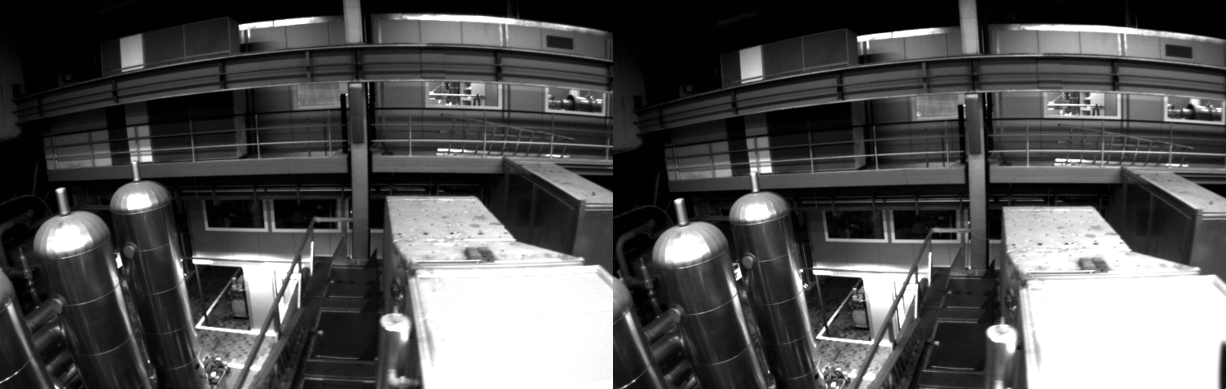
\includegraphics[width=14.5cm]{毕设图片/3-8}
%     \caption{\label{fig:3-8}EuRoC数据集中的双目图像}
% \end{figure}
% \begin{figure}[H]
% \centering %将图片居中显示
%     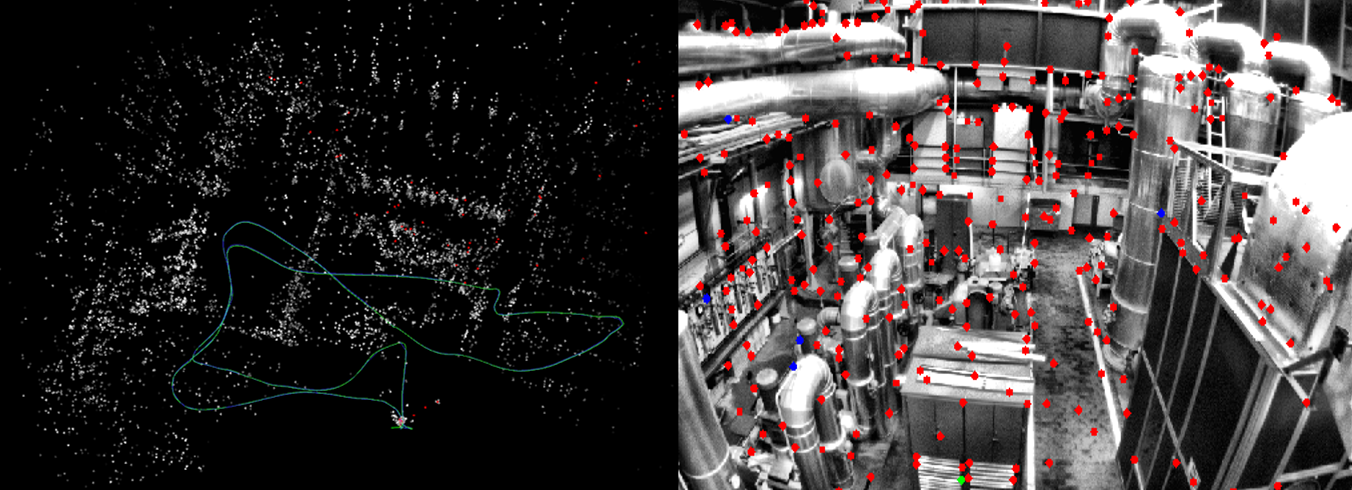
\includegraphics[width=14.5cm]{毕设图片/3-9}
%     \caption{\label{fig:3-9}RRVIP-SLAM在EuRoC数据集的运行效果}
% \end{figure}



% VIO部分的测试结果如\autoref{tab:4}所示,本文所提出的算法均为运行5次取得的平均值,作对比的算法均采用其发表论文中所给出的测试结果。使用本数据集测试时,测试的各个算法均能运行完全程,完成度均为100\%,故不列出完成度。\autoref{fig:3-10}展示了各个算法在MH\_05序列上路径和xyz坐标方向的轨迹误差。

% \begin{table}[H]
%     \fangsong
%     \caption{\label{tab:4}各算法在EuRoC中MH数据集上的测试结果}
%     \small %此处写字体大小控制命令
%     \centering%把表居中
%     \renewcommand{\arraystretch}{1.5}
%     \setlength{\tabcolsep}{3mm}{
%     \begin{tabular}{ccccc}
%     \toprule%第一道横线
%      & VINS-Fusion & ORB-SLAM3 & OV2-SLAM & RRVIP-SLAM  \\ 
%     \midrule%第二道横线 
%     MH\_01 & 0.166 & 0.036 & 0.054 & 0.044 \\
%     MH\_02 &	0.152 &	0.033 &	0.041 & 0.037 \\
%     MH\_03 &	0.125 & 0.035 &	0.058 &	0.042 \\
%     MH\_04 &	0.280 &	0.051 & 0.116 &	0.076 \\
%     MH\_05 &	0.284 &	0.082 &	0.140 &	0.065 \\
%     \bottomrule%第三道横线
%     \end{tabular}}
% \end{table}

% \begin{figure}[H]
%     \centering
%     \subfigure[{\fangsong 总体轨迹展示}] {\includegraphics[width=7.25cm,height = 6.5cm]{毕设图片/euroc_traj.png}}%
%     \subfigure[{\fangsong 各方向轨迹展示}] {\includegraphics[width=7.25cm,height = 6.5cm]{毕设图片/euroc_ape.png}}
%     \caption{\label{fig:3-10}各算法在EuRoC MH\_05计算轨迹结果}
% \end{figure}

% 通过对比发现,相对于改进前的OV2SLAM算法,RRVIP-SLAM定位精度有了明显的提升,并且相比较于主流VIO算法,本文提出的算法具有相同水平的高精度。


% \subsection{Aqualoc数据集测试}
% 该数据集包括两个部分,300米左右水深的考古场景Archeological数据集和港口Harbor数据集,如\autoref{fig:3-11}所示。本文使用其中的考古场景数据集进行测试,为了能在该数据集上测试,本文在算法中添加了单目惯性深度融合模块。单目相机紧耦合算法参考了Vins-Mono算法\cite{VINSMono}中的方法,在本文的双目紧耦合算法中去掉了右相机并添加了单目尺度信息;并在算法初始化时参考了原始的OV2SLAM算法,使用单目相机对极几何计算出单目图像之间的相对位姿,并在初始化紧耦合优化中使用IMU提供的尺度进行对齐。
% \begin{figure}[H]
%     \centering
%     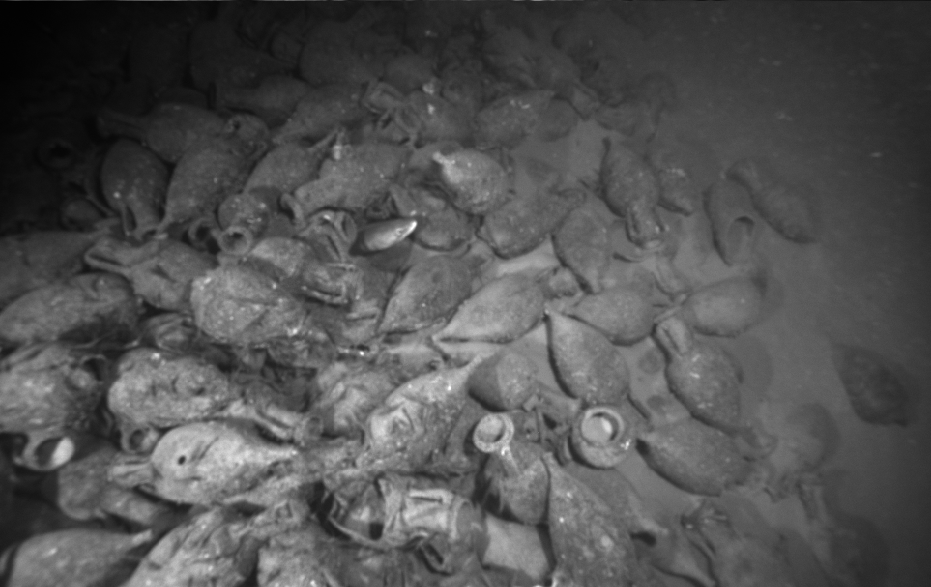
\includegraphics[width=7cm]{毕设图片/3-11}
%     \caption{\label{fig:3-11}Aqualoc数据集图像}
% \end{figure}

% RRVIP-SLAM算法在水下考古场景中的结果如\autoref{fig:3-12}所示,\autoref{fig:3-13}与\autoref{tab:4-2}展示了各个算法的ATE误差和完成度,相较于主流VIO算法,RRVIP-SLAM算法鲁棒性更好,主流VIO算法在很多测试场景中发生了初始化失败、跟踪丢失、IMU漂移等问题,且超过了VINS-Fusion在水下场景中的精度。相较于改进之前的OV2SLAM算法,本文通过添加IMU和深度计,IMU与相机实现互补计算,在特征点较少时,会使用惯性进行导航,保证短时间内不会跟丢,使得在水下场景中的稳定性大大提高,在4个序列中的3个都运行完全程,序列4中场景过于浑浊,所有算法均失效。\autoref{fig:3-12}左图为RRVIP-SLAM在Arch\_06序列上的运行效果,稳定地运行完了全程的轨迹。\autoref{fig:3-12}右图展示了在水下考古场景中,即使在较平整的地面上,RRVIP-SLAM算法也能稳定地跟踪到特征点。
% \begin{figure}[H]
%     \centering
%     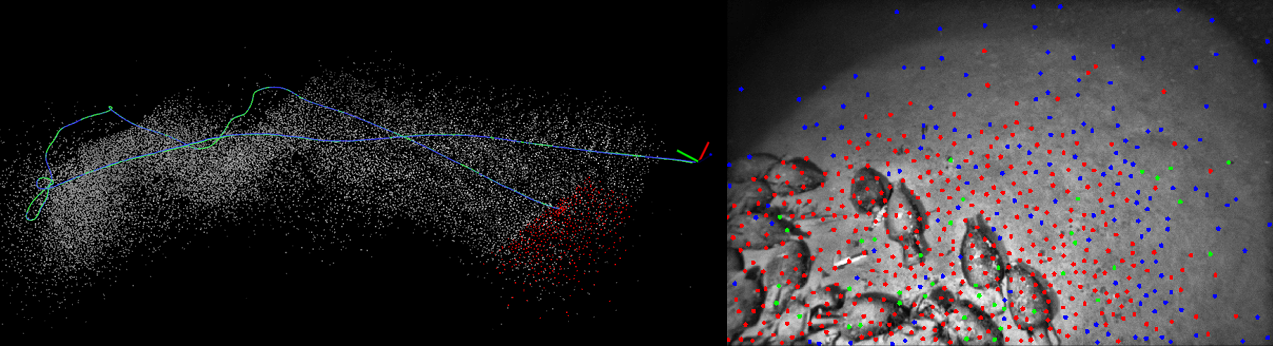
\includegraphics[width=14.5cm]{毕设图片/3-12}
%     \caption{\label{fig:3-12}RRVIP-SLAM在Arch\_06数据集的运行效果}
% \end{figure}



% \begin{figure}[H]
%     \centering
%     \subfigure[{\fangsong 总体轨迹展示}] {\includegraphics[width=7.25cm,height = 6cm]{毕设图片/aqua_traj.png}}%
%     \subfigure[{\fangsong 各方向轨迹展示}] {\includegraphics[width=7.25cm,height = 6cm]{毕设图片/aqua_traj2.png}}
%     \caption{\label{fig:3-13}各算法在Arch\_05计算轨迹结果}
% \end{figure}



% \begin{table}[H]
%     \fangsong
%     \caption{\label{tab:4-2}各算法在Aqualoc数据集上的测试结果}
%     \small %此处写字体大小控制命令
%     \centering%把表居中
%     \renewcommand{\arraystretch}{1.5}
%     \setlength{\tabcolsep}{3mm}{
%     \begin{tabular}{cccccc}
%     \toprule%第一道横线
%     & & VINS-Fusion & ORB-SLAM3 & OV2-SLAM & RRVIP-SLAM  \\ 
%     \midrule%第二道横线 
%     \multirow{2}{*}{Arch\_04} & ATE & $ \times $ & $ \times $ & $ \times $ & $ \times $ \\
% 			% \cline{2-5}
% 			& 完成度 & 0\% & 0\% & 0\% & 0\% \\
%     % \midrule%第二道横线 
%     \multirow{2}{*}{Arch\_05} & ATE  & 1.56 & $ \times $ &0.119 & 0.077 \\
% 			% \cline{2-5}
% 			& 完成度 & 100\% & 0\% & 55.8\% & 100\% \\
%     % \midrule%第二道横线 
%     \multirow{2}{*}{Arch\_06} & ATE  & 3.77 & $ \times $ & 1.509 & 0.188 \\
% 			% \cline{2-5}
% 			& 完成度 & 100\% & 0\% & 60.1\% & 100\% \\
%     % \midrule%第二道横线 
%     \multirow{2}{*}{Arch\_07} & ATE  & $ \times $ & 0.718 & 0.548 & 0.550 \\
% 			% \cline{2-5}
% 			& 完成度 & 0\% & 37.8\% & 35.1\% & 100\% \\
%     \bottomrule%第三道横线
%     \end{tabular}}
% \end{table}



% \subsection{Cave数据集测试}
% Cave数据在美国佛罗里达州附近拍摄,全长155米,该数据集使用了双目相机、IMU和深度传感器,匹配RRVIP-SLAM算法测试需求。\autoref{fig:3-14}展示了该数据集中双目相机所拍摄的图片,拍摄于海底的一个洞穴。该数据集体现了水下环境的特殊性:环境黑暗、有漂浮的杂质。

% \begin{figure}[H]
%     \centering
%     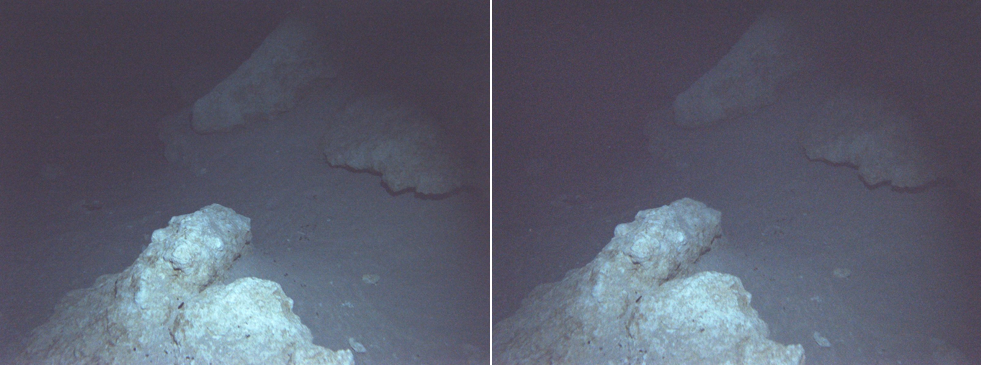
\includegraphics[width=14.5cm]{毕设图片/3-14}
%     \caption{\label{fig:3-14}Cave数据集双目相机图像}
% \end{figure}

% \autoref{fig:3-15}展示了RRVIP-SLAM算法在洞穴场景中运行的效果,前端跟踪和后端优化计算出的轨迹分别为绿线和蓝线,之所以两条曲线有较大偏移,是因为本算法使用词袋模型检测到了再次经过的位置,使用闭环优化消除了算法的累积误差,在回环后将轨迹纠正到了正确的位置上。\autoref{fig:3-15}右图为本算法的前端在水下洞穴场景中跟踪到的特征点。


% \begin{figure}[H]
%     \centering
%     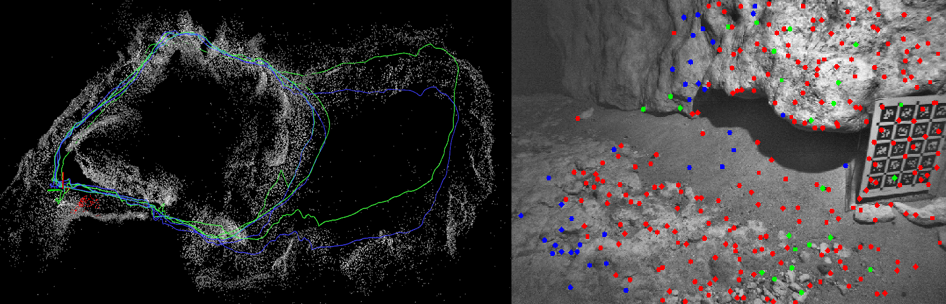
\includegraphics[width=14.5cm]{毕设图片/3-15}
%     \caption{\label{fig:3-15}RRVIP-SLAM在Cave数据集的运行效果}
% \end{figure}

% 本文在Cave数据集上对比了当前流行的VIO算法和改进前的OV2SLAM算法,\autoref{fig:3-16}和\autoref{tab:5}展示了对比结果。可以看出,RRVIP-SLAM算法完成度最高,精度属于较高水平,在三个方向的坐标上均与轨迹真值贴合的很好,而其他三种算法均未完成轨迹跟踪,在运行一段路程后或者在初始场景中跟踪丢失。其中,ORB-SLAM3算法在初始路程中精度较高,但其跟踪丢失较快,并不适用于水下场景;而相较于OV2SLAM算法,本文通过融合IMU和深度信息,使得算法在鲁棒性和精度上有明显提升。


% \begin{figure}[H]
%     \centering
%     \subfigure[{\fangsong 总体轨迹展示}] {\includegraphics[width=7cm,height = 5cm]{毕设图片/cave_traj.png}}
%     \subfigure[{\fangsong 各方向轨迹展示}] {\includegraphics[width=7cm,height = 5cm]{毕设图片/cave_traj2.png}}
%     \caption{\label{fig:3-16}各算法在Cave计算轨迹结果}
% \end{figure}


% % \begin{figure}[H]
% %     \centering
% %     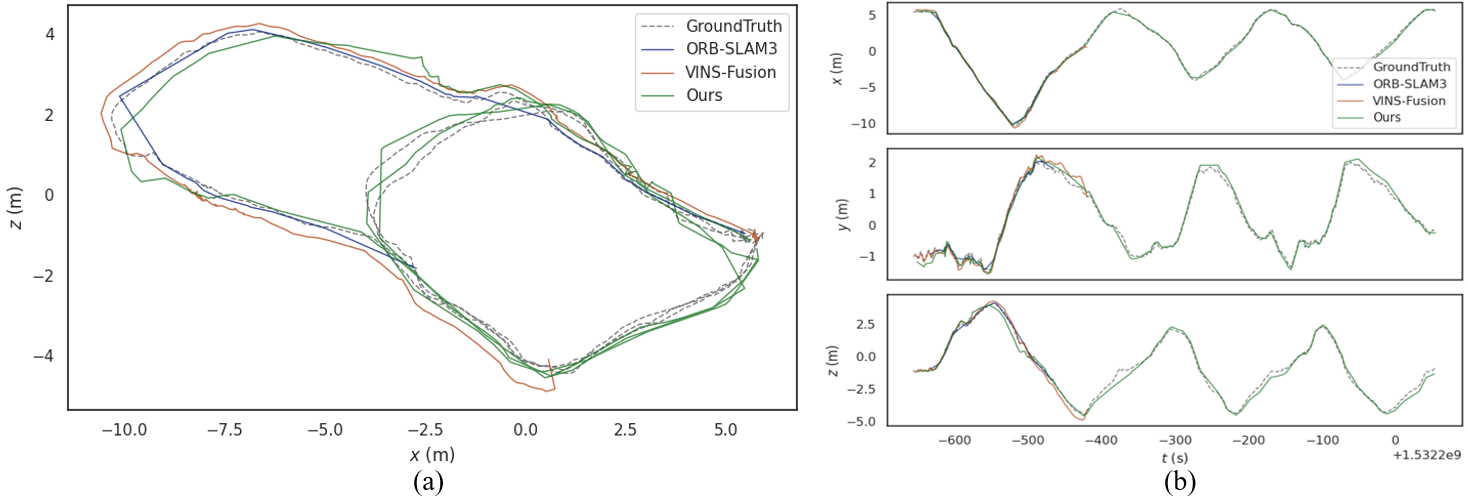
\includegraphics[width=14.5cm]{毕设图片/3-16}
% %     \caption{\label{fig:3-16}各算法在Cave计算轨迹结果(a)总体轨迹展示(b)各方向轨迹展示}
% % \end{figure}
% \begin{table}[H]
%     \fangsong
%     \caption{\label{tab:5}各算法在Cave数据集上的测试结果}
%     \small %此处写字体大小控制命令
%     \centering%把表居中
%     \renewcommand{\arraystretch}{1.5}
%     \setlength{\tabcolsep}{3mm}{
%     \begin{tabular}{ccccc}
%     \toprule%第一道横线
%      & VINS-Fusion & ORB-SLAM3 & OV2-SLAM & RRVIP-SLAM  \\ 
%     \midrule%第二道横线 
%     完成度 & 34.5\% & 29.1\% & 0\% & 100\% \\
%     ATE & 0.34 & 0.09 & $ \times $ & 0.32 \\
%     \bottomrule%第三道横线
%     \end{tabular}}
% \end{table}


% \section{本章小结}
% 本章提出了一种适用于水下场景的“双目视觉-惯性-深度”紧耦合位姿计算方法,通过分析相机、IMU和深度计的物理特性和计算残差矩阵,将各传感器的残差统一变换至体坐标的位姿,用于联合优化。在此基础上,分别在SLAM领域常用的空气中EuRoC数据集和水下数据集Aqualoc和Cave测试,通过比较本文算法和现有主流VIO算法以及OV2SLAM算法,定量分析证明了RRVIP-SLAM算法在水下场景中的高精度和稳定性。然而,公开数据集没有考虑水下折射畸变,且未给出相机折射参数,本章只能进行定位定姿算法间的横向比较。在后续水池试验章节中,将进一步验证水下折射畸变校正对定位定姿的有效性。